\documentclass[11pt]{report}

\usepackage{graphicx}
\usepackage{float}
\usepackage[parfill]{parskip}
\usepackage{rotating}
\usepackage{listings}
\usepackage{flafter} 
\usepackage{color}
\usepackage{cite}
\usepackage[round]{natbib}
\usepackage{comment}
\usepackage{color}
\usepackage{listings}
\usepackage{setspace}
\usepackage[toc,page]{appendix}

\definecolor{Code}{rgb}{0,0,0}
\definecolor{Decorators}{rgb}{0.5,0.5,0.5}
\definecolor{Numbers}{rgb}{0.5,0,0}
\definecolor{MatchingBrackets}{rgb}{0.25,0.5,0.5}
\definecolor{Keywords}{rgb}{0,0,1}
\definecolor{self}{rgb}{0,0,0}
\definecolor{Strings}{rgb}{0,0.63,0}
\definecolor{Comments}{rgb}{0,0.63,1}
\definecolor{Backquotes}{rgb}{0,0,0}
\definecolor{Classname}{rgb}{0,0,0}
\definecolor{FunctionName}{rgb}{0,0,0}
\definecolor{Operators}{rgb}{0,0,0}
\definecolor{Background}{rgb}{0.98,0.98,0.98}

\lstnewenvironment{python}[1][]{
	\lstset{
		numbers=left,
		numberstyle=\footnotesize,
		numbersep=1em,
		xleftmargin=1em,
		framextopmargin=2em,
		framexbottommargin=2em,
		showspaces=false,
		showtabs=false,
		showstringspaces=false,
		frame=l,
		tabsize=4,
		% Basic
		basicstyle=\ttfamily\small\setstretch{1},
		backgroundcolor=\color{Background},
		language=Python,
		% Comments
		commentstyle=\color{Comments}\slshape,
		% Strings
		stringstyle=\color{Strings},
		morecomment=[s][\color{Strings}]{"""}{"""},
		morecomment=[s][\color{Strings}]{'''}{'''},
		% keywords
		morekeywords={import,from,class,def,for,while,if,is,in,elif,else,not,and,or,print,break,continue,return,True,False,None,access,as,,del,except,exec,finally,global,import,lambda,pass,print,raise,try,assert},
		keywordstyle={\color{Keywords}\bfseries},
		% additional keywords
		morekeywords={[2]@invariant},
		keywordstyle={[2]\color{Decorators}\slshape},
		emph={self},
		emphstyle={\color{self}\slshape},
		%
	}}{}

\lstset{frame=tb,
  aboveskip=3mm,
  belowskip=3mm,
  showstringspaces=false,
  columns=flexible,
  basicstyle={\small\ttfamily},
  numbers=none,
  breaklines=true,
  breakatwhitespace=true,
  tabsize=3
}
\usepackage{fancyhdr}
\setlength{\topmargin}{-.5in}
\setlength{\textheight}{9in}
\setlength{\oddsidemargin}{.125in}
\setlength{\textwidth}{6.25in}
\graphicspath{images/}
\begin{document}
\title{An Investigation into Network Emulation as a Testing Platform}
\author{Robert Game}
\date{}
\maketitle

\chapter*{Abstract}

In recent years technology for large enterprise has advanced significantly due to the introduction of virtualisation of infrastructure. This has allowed even the smallest of enterprise to adopt low-cost, virtual copies of their Production servers as a test bed and facilitates the segregation of Production and Development by holding a copy of the Production server for testing in Pre-Production. This means that when planning changes to a server it can first be tested in order to ensure that no unanticipated issues occur. This practise has been well adopted on the server infrastructure, however, when looking at network infrastructure there has not been significant uptake in the use of virtualisation to facilitate testing in this way. Many Network Operations teams rely on the use of a physical lab for the testing of changes, however these labs take considerable time to set up both from a cabling perspective and from configuring each device. This project aims to investigate more efficient methods of testing network changes through the use of router virtualisation. In order to do this I will investigate the Cisco's new product VIRL and how it can be used to create a tool which will provide a testing platform for network changes. In addition to simulating the network infrastructure this project will also investigate meaningful methods of creating testing evidence for use in large infrastructure. When implementing network changes in large infrastructure this is particularly useful evidence to have as Change Management teams continuously seek to avoid risk.

\pagebreak

\tableofcontents

\chapter{Introduction}

In recent years the use of a second, entirely separate infrastructure has been used to develop tools, test changes and simulate outages of IT Systems. In a large scale infrastructure these environments are usually created for testing changes on Server or Application environments, however the need for real traffic and the cost of dedicated hardware makes this difficult in the Network Infrastructure. The use of a physical lab takes time to set up and teams usually do not use them unless they are planning for large scale infrastructure changes.

This project will aim to create a tool intended for use in a Network Operations team in large scale enterprise. This tool will aim to pull together different aspects of Network Management tools and use information available to create a network model inside of the Cisco VIRL emulated environment. Using this model the Network Operations team can test environment changes on a model of their own network. Using data gathered from this simulation and the changes observed during any configuration edits the tool will then aim to create a piece of testing evidence which can be used to support any Change Management required on the infrastructure.

Large organisations, which are the primary target of the proposed tool, will often have Configuration Repositories and Configuration Management Databases (CMDB) that store relevant configurations and server locations. Alternatively, a networks team may want to generate a emulated version of an unknown network in order to understand its topology and configuration. The proposed tool will combine network emulation technology with these data sources to allow an Administrator to mimic changes to a production network and observe the impact that they have on data flow and connectivity. In particular the tool will generate testing evidence as proof of any impact (or lack of) when raising a network change.

The proposed tool provides value to a Network Engineer as it allows them to be more flexible in their network testing. With the proposed solution an Engineer will no longer need to create a physical clone of the network in a lab environment, nor will the need rely on outdated documentation. A emulated copy of the network can be produced from a node-edge representation of the topology along with the configurations for devices. This will save the Engineer time in the planning as well as allowing them to implement the changes in a non-production environment, in addition to the time savings an Engineer will also be able to produce testing evidence which can be used for Change Management purposes.

From initial findings it is understood that there are currently solutions for creating a simulated network, however, these tools rely on an Engineer to rebuild a network from scratch. Implementing the topology and interconnecting devices requires a well-documented network and in addition to the physical layout, the simulated devices also require a configuration which matches the real network. This project will aim to create a tool which will provide use to a Network Engineer regardless of the documentation they have for their infrastructure, allowing the Engineer to produce an emulated copy of their physical network without the need to reproduce the infrastructure on a device-by-device basis. The tool will produce an emulation of the network as a whole rather than focusing on devices.

\section{Scope}

This solution is targeted at medium to large enterprise which have a considerable routing set-up For example a global or regional backbone which connects multiple branch offices to a Headquarters. My tool will support both Interior and Exterior Routing protocols. In particular I am using my experience in the finance industry where Network Operations teams also work in an ISP role connecting through EBGP as well as traditional interior Distance Vector or Link State routing. This will create a tool that is scalable to the users needs, allowing a user to create a emulated copy of their local network through dynamic device discovery or a larger scale Engineer to produce an emulated version of a section of their network using Configuration Repositories and Network Diagrams.

\section{Objectives}
\begin{itemize}
\item{Create a tool which can take information from existing resources and create a working model of the Network Infrastructure within Cisco VIRL.}
\item{Extend the tool so that it can dynamically discover new network devices.}
\item{Facilitate the creation of a simulation within five minutes of starting the tool.}
\item{Produce a visual representation of the network for the user to view}
\item{Allow the user to interact with the emulation through traditional methods such as SSH or telnet}
\item{Investigate new methods for an Engineer to interact with a network}
\item{The production of detailed testing evidence during the simulation, such as neighbour tables, routing entries or link statuses.}
\end{itemize}

\chapter{Literature Review}

This chapter will review current publications in the field of network simulation and testing, I will use this literature first to gain inspiration for this project but also as a gap-analysis of the proposed tool. It will first focus on the use of Virtualisation in computer infrastructure, before looking at the use of network management techniques to gather information about a the infrastructure before finally focusing on 'What-if?' scenarios on a network and which tests are of most beneficial to a Network Engineer.


\section{Virtualisation of Infrastructure}

Virtualisation of infrastructure components has grown rapidly in the previous decade with the implementation of Cloud Computing being ``one of the most explosively expanding
technologies in the computing industry today'' \citep{younge2011analysis}.

The technology relies on creating a sandbox within a physical host in which ``multiple operating systems can safely coexist on one physical machine'' \citep{mergen2006virtualization} these virtual operating systems are governed by a tool known as a Hypervisor or Virtual Machine Monitor which ``safely multiplexes the hardware resources of the physical machine but leaves the specific hardware resource allocation to the operating system in the virtual machine'' \citep{mergen2006virtualization} creating the illusion to these virtual operating systems that they have full control of their hardware when in fact they are running in a sandbox environment cut-off from the 'real' hardware. 

The benefits of server virtualisation come in both a technical and economic form. \citep{crosby2006virtualization} says ``the artifacts of current operating-system and system-software architecture result in most servers today running at under 10 percent utilization.'' from a technical perspective the implementation of a virtual server for multiple operating system instances versus a separate physical host each allows for much better utilisation of a single server and thus provides gains in capacity management for infrastructure. Economic benefits come from the amount of physical hardware required in a Data Centre, \citep{daniels2009server} says ``Data center floor space and rack space are prime real estate in computing environments. Cooling and electricity costs have risen in recent years'' and the adoption of virtual infrastructure can help keep costs down which allows enterprises to implement practises such as High Availability services.

At first glance the adoption of virtual infrastructure may seem to only bring benefits to enterprise, however \citep{kotsovinos2010virtualization} highlights some issues that arise with implementing virtualisation technology in large infrastructure. In this article the author talks about issues such as System Sprawl where `developers forget to return the VMs they do not use to the pool after the end of a project' creating problems in accountability and server ownership. In addition to this there is also a breakdown in the conventional responsibility of teams (silos) as issues can arise from multiple areas of infrastructure, the author says `cross-silo collaboration and communication are of paramount importance, requiring a true mentality shift in the way enterprise infrastructure organizations operate' which may be difficult to implement. A third issue that arises is the added complexity of changes as `Sharing the infrastructure comes with centralization and, therefore, with potential bottlenecks that are not as well understood' this creates additional complexity in Change Management as it is no longer as clear how a decision can affect the infrastructure as a whole.

From the literature it is clear that virtualisation is a technology which is gaining momentum in large enterprise. The use of which allows engineers to make use of their infrastructure efficiently in both capacity and cost. It is clear that virtualisation is the correct method of implementing a network testing tool due to its scalability and ease of implementation when compared to physical equipment. 

\section{Virtualisation of Network Components}

From a testing perspective, virtualisation in the network infrastructure comes in the form of device emulation. \citep{galan2004use} discusses the use of virtualisation tools within a network lab, 
in this paper the author describes a scenario in which they have used a virtual network as a platform for learning. Features such as the ability to quickly create a simulation and the ease of restoring defaults when problems arise are highlighted as a significant benefit of simulation over real devices, particularly in a learning environment where misconfigurations are likely to occur. However, the author also highlights opportunities that are missed with simulated devices, such as having no physical contact with the routers means that hands-on experience is lost.

\citep{Knight:2012:ASL:2342356.2342378} says ``Emulated networks, which run a real router operating systems inside virtual machines, offer realistic yet inexpensive network experimentation. However they are time-consuming to configure, which limits their use in network research''. In this paper there is a proposal of a tool to simplify the creation of emulated networks, Autonetkit, which provides the ability to generate thousands of lines of configuration code across multiple devices from a high-level description of the topology as a whole. In particular this paper highlights the difficulty faced when creating an emulated network from scratch. When dealing with networks of hundreds or possibly thousands of nodes the time taken to configure each can outstrip the benefits of an emulated network.

This section of the Literature Review has given views on both the benefits and shortfalls of using virtualisation in network infrastructure. A significant benefit to network emulation is cost, with physical devices there is a significant investment in a single device with most requiring a support contract. For a large organisation this may be seen as an unnecessary expenditure, whereas the licensing cost for a VM may be considerably more cost effective. One shortfall of emulation that has been identified in the literature is the difficulty of defining a network from scratch, this will be taken into consideration when designing the proposed solution.

\section{Network Management and What-if? Scenarios}

Configuration and Change Management is a particularly important aspect in modern infrastructure systems, in particular improved vigilance on Change Management to Networks can improve reliability and uptime in for systems as a whole. \citep[p.270-273]{bellovin2009configuration} discusses these aspects both from a network and whole infrastructure perspective. In the paper's case study it talks of the importance of router configuration management to a large Internet Service Provider, one particular use of configuration management is understanding a malicious attack by viewing the current configuration as `the differences between the authorized configuration and the one installed by the intruder can give valuable clues as to goals and motives'

`What-if' scenarios are a section of Network Testing that allows an Engineer to understand how their topology will cope should an event occur. \citep{lad2006visualizing} discusses a potential solution to the uncertainty of a network change on the Internet, in this paper the author proposes a tool which allows the impact of a BGP update to be understood by providing a visual representation of changes to an Autonomous System's forwarding path. This tool allows an Engineer to understand where traffic is flowing in the event of a change to a network. However, this tool falls short as it only allows an Engineer to view routing changes in real-time instead of gaining an understanding of what could happen.

This section of the Literature Review was particularly difficult as there are very few tools available that allow both emulation of a real network and feedback on changes to the emulated network. This indicates a gap in current solutions which the proposed solution may be able to target.

\chapter{Current Solutions and Cisco VIRL}

\section{Current Solutions}

\subsection{Hardware}

Traditional approaches to Network Testing would rely on hardware to be a `true' copy of the Production Network. However as infrastructure grows and becomes more complex, the flexibility of this method diminishes. The use of hardware for testing relies on an organisation having a complete network lab on-site which an Engineer can use to build smaller sections of the Production network, replicating the topology by using identical device models to the production counterpart along with the same software version and running configuration. This creates an additional burden on any proposed changes to a Production network as every change requires a physical build of a clone of the network before testing can occur. In addition to the time cost associated with this testing, there is an additional monetary cost to an organisation as they need to hold additional hardware, usually with a large support contract attached, in order to be able to carry out testing. For some smaller enterprise this additional cost may not be viable and some risks may be taken by implementing changes without prior testing.

\subsection{Simulation}

Network Simulation extends the concept of testing by allowing a user to create a simulated network, however, this is not full emulation and is not as reliable as a testing tool when compared to other methods. In recent years simulation of networks has been used as a tool for vendor-specific educational courses such as Cisco's CCNA or Juniper's JNCIA certification programs.

Cisco's offering on the simulation market is an educational tool for basic learning of the Cisco Certified Network Associate (CCNA) certification. Packet Tracer \citep{ciscoPacketTracer} takes form as a topology view which allows a user to drag and drop routers and switches onto the topology. The devices run a simplified version of the Cisco IOS and allow the user to connect to the devices serial port in order to configure them. An example of Packet Tracer is shown in Figure 3.1.

\begin{figure}[h!]
	\caption{Cisco Packet Tracer}
	\centering
	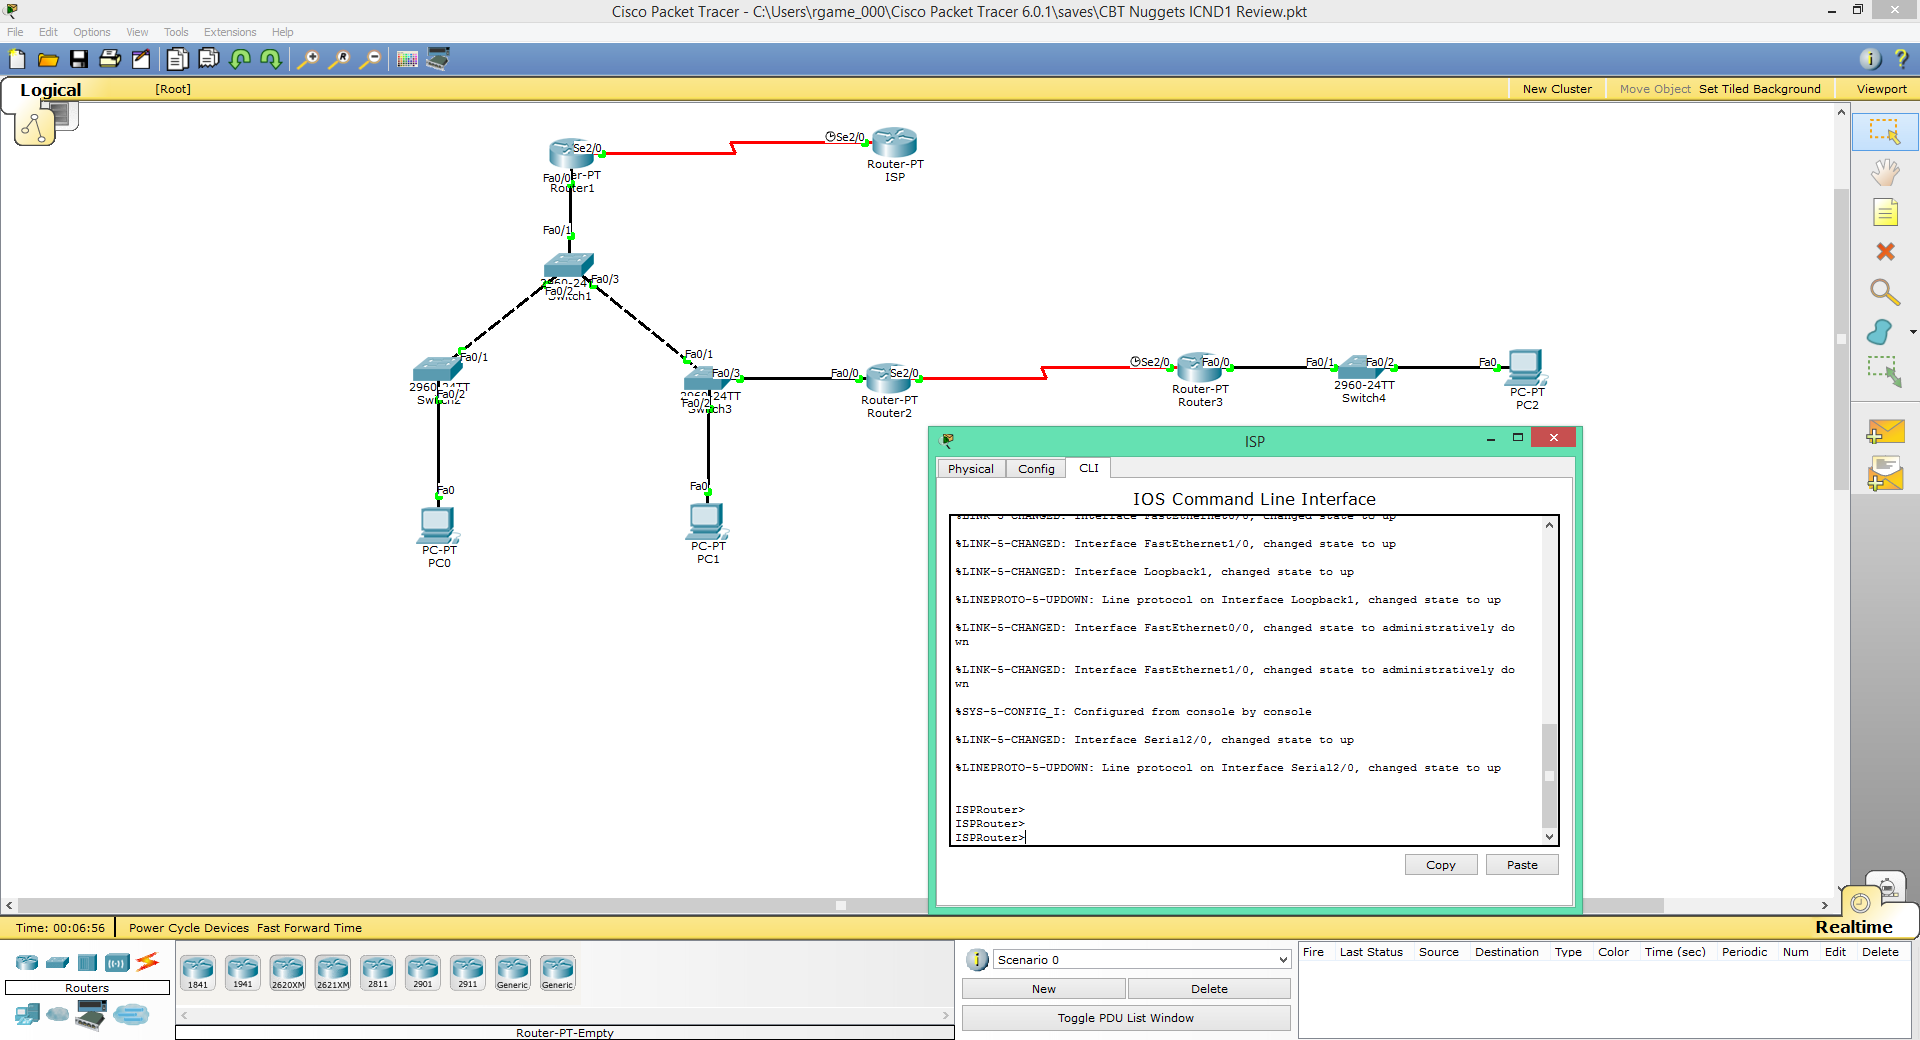
\includegraphics[width=1\textwidth]{packetTracer.png}
\end{figure}

 These simulations tend to focus on creating a learning environment for their tools and as such do not perform adequately as simulated `real world' devices. These devices tend to work as a simulator in that they mimic the behaviour of a network, and not the devices. For example, the software will decide to build an OSPF neighbouring should the required fields match on the devices. In contrast, a simulator (and real device) will build the relationship through a series of negotiations and packet transfers. As a result these simulators cannot be used reliably as network testing tool as the behaviour is predefined and may not be a true reflection of real hardware.
 
 Other network device vendors such as Juniper, HP and Huawei have offered simulated versions of their network equipment which work on similar principals, however these tools have not been a focus of this section as they do not emulate Cisco software.

\subsection{Emulation}

The Open Source community has also played a role in this virtual networks field, a project named GNS3 \citep{GNS31.2} was started in 2006 which aimed to create  unified tool to pull together hardware simulation and topology design into one UI. From this they created GNS3, a front end which allowed users to create a topology in a ‘drag and drop’ style and then start equipment as required. GNS3 is intended to be a multi-vendor tool but is particularly used for Cisco simulations. Using a hypervisor called Dynamips the tool can create a VM of a Cisco router which can be interconnected to create a real topology. In addition to this, GNS3 can be adapted as a network emulator, which enables a user to connect their simulated topology to their physical network.

\begin{figure}[h!]
	\caption{GNS3 1.2}
	\centering
	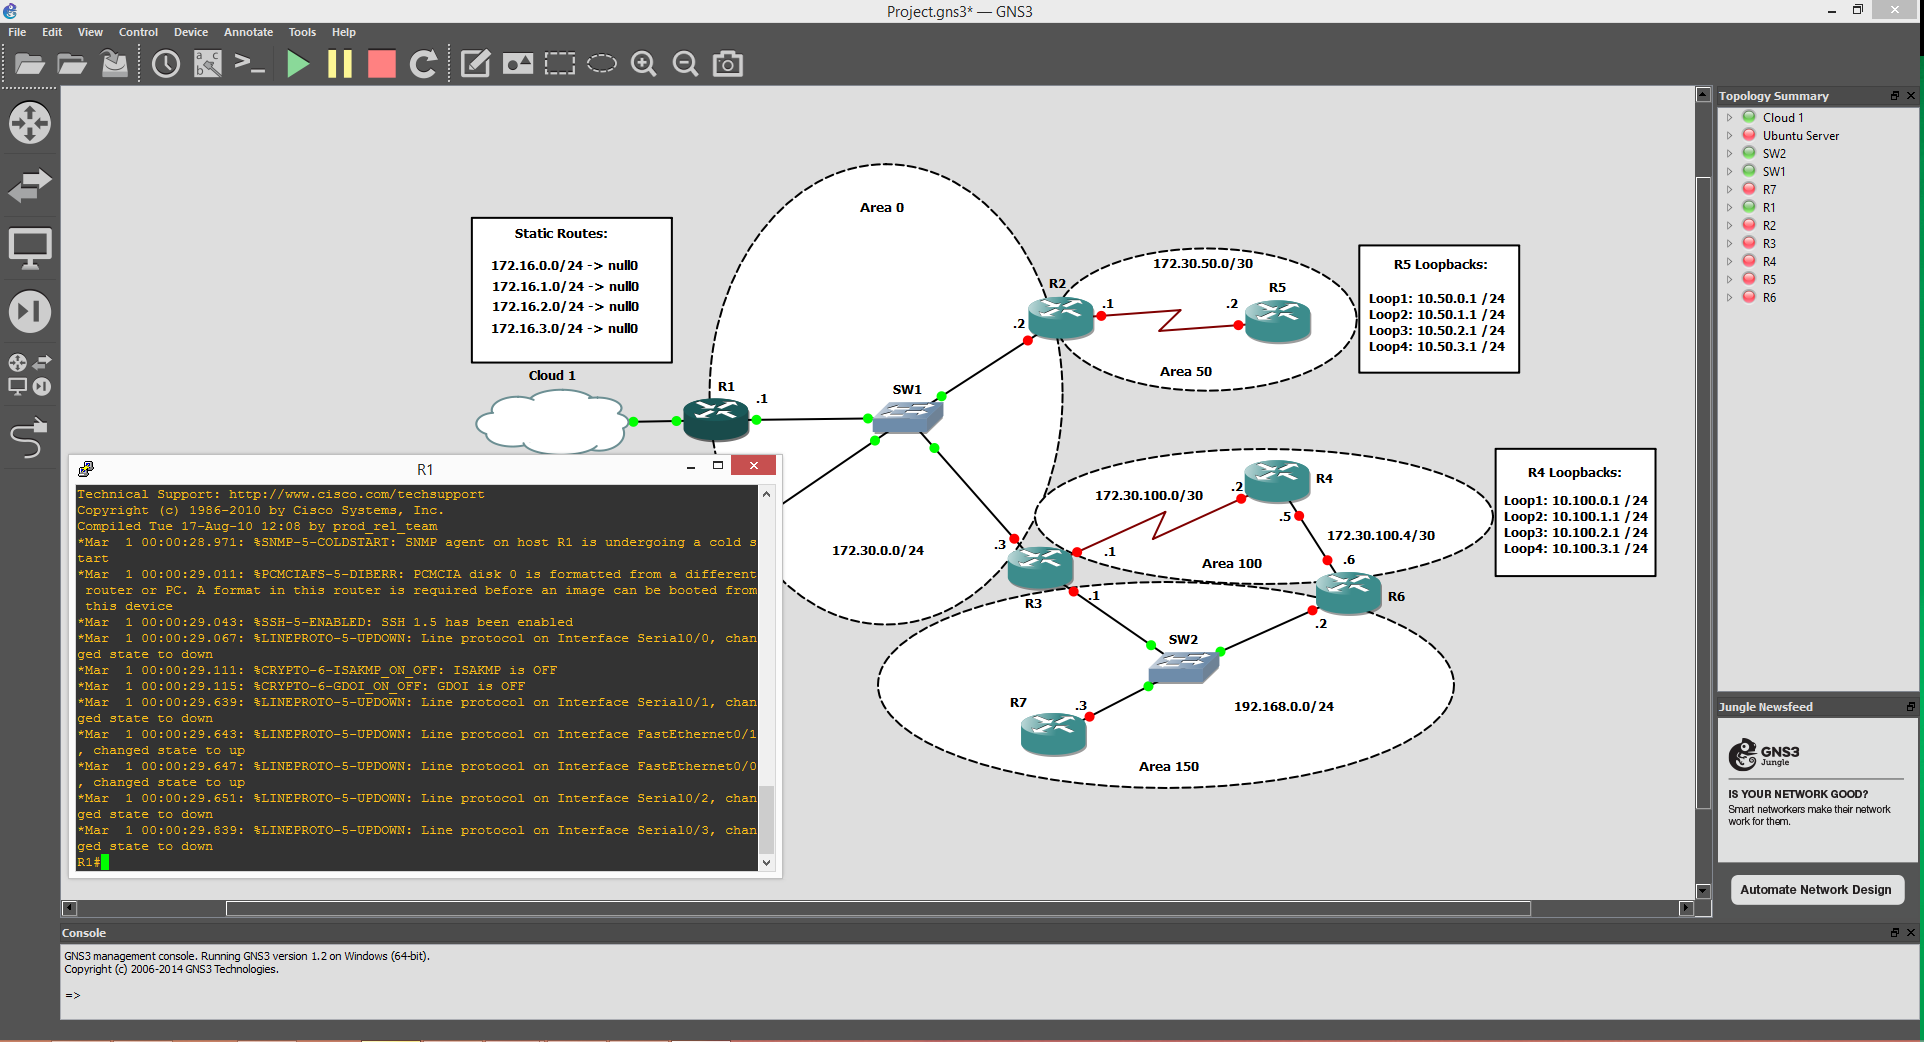
\includegraphics[width=1\textwidth]{GNS3.png}
\end{figure}

GNS3 works well for Cisco router simulation, however it falls short when looking at Layer 2 simulation. Features such as Spanning Tree Protocol rely heavily on the fast processing speed of Application Specific Integrated Circuitry (ASICs) which are controllers within the switches that can quickly process frames. Cisco IOS combined with Dynamips cannot process frames fast enough in order to successfully implement these protocols. Therefore when testing redundancy scenarios such as outages which force a Layer 2 topology change cannot be tested. In addition to the issues outlined above there is no support for network discovery and the building of topologies for network testing.

In addition to the shortfalls in some protocols, GNS3 lacks the scalability of some of its competitors. On a conventional PC it can emulated 10-15 devices, however may use up to 90\% of the host's CPU if the IOS version is not calibrated for the host PC, because of this lack in scalability it may not be of any use to large enterprise.

From the review of current solutions there has not been a tool which can generate simulations of existing hardware. The only solutions at current are bare-bones building tool for network designs. The proposed tool is different in that its purpose is to be used in existing infrastructure to test disaster recovery or planned configuration changes.

\section{Cisco Virtual Internet Routing Lab (VIRL)}

Cisco VIRL is a relatively new offering on the Virtualisation market, VIRL is pre-release software which forms the back end for a future Cisco product called Cisco Modelling Labs. This tool provides emulation using a new version of Cisco’s IOS and NexusOS, tailor made for virtualisation and fast deployment.

VIRL is a relatively new offering from Cisco, and is their first software specifically created to support virtual copies of their routers. It was first released to the public in November 2014 as a stand-alone client installed on a local machine. However for the purposes of this Project I have been fortunate enough to have access to the University's own server-based version of VIRL. This provides support for up to 200 instances in comparison to the Personal Edition which is capped at 15 instances. This has enabled me to take advantage of extra features such as Servers which can be attached to a network topology, providing added features such as network analysis and traffic creation.

\begin{figure}[h!]
	\caption{Cisco VM  Maestro}
	\centering
	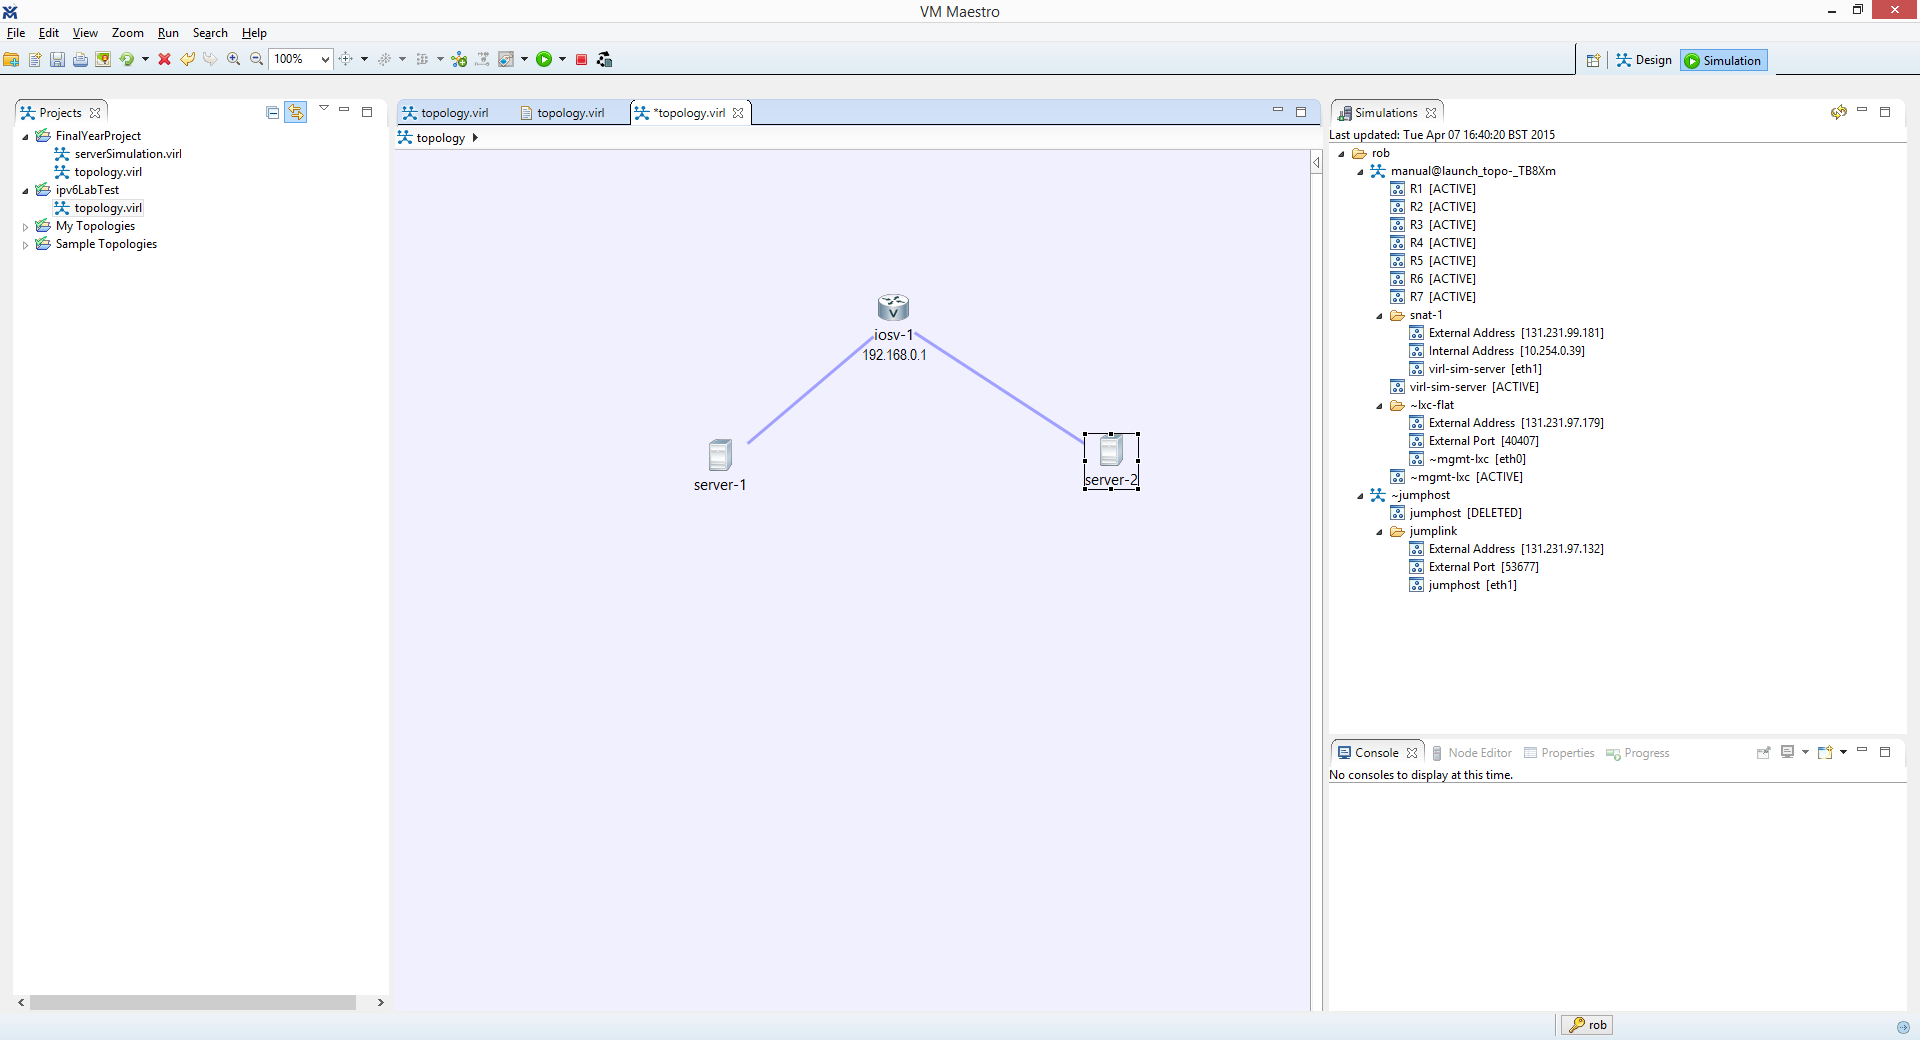
\includegraphics[width=1\textwidth]{VIRL.png}
\end{figure}

Connection to the VIRL Server is provided though an Eclipse-based front-end called VM Maestro. This interface provides an sandbox to build network topologies using the provided images of Cisco hardware within VIRL. For this project I will be concentrating on the use of Cisco's IOSv image, an image of the traditional IOS but adapted for use with a hypervisor. This allows the image to be run on a server without any dedicated ASICs. VIRL can then interconnect these devices provide connectivity and traffic. Using these connections the Routers can use routing protocols such as OSPF, EIGRP or BGP in order to create routing tables - this enables the user to simulate the Layer 3 functionality of their topology.

VIRL has also been designed with flexibility in mind for its users, one specific feature of note is the support of a tool called Autonetkit. This integration allows VIRL to create a fully functioning topology in a matter of seconds as configurations such as ip addressing and routing protocols can be passed off to Autonetkit which will auto-generate a working topology.

In addition to the features provided for functionality within VM Maestro, there are also a variety of configurations available to connect VIRL to the outside world. The first available connection is FLAT Networking - this provides a layer 2 interface which can bridge VIRL with physical hardware. This is particularly useful as it allows a user to integrate Layer 2 functionality with their simulation, an area in which VIRL is currently lacking. The second method of connectivity is through a SNAT connection on the VIRL simulation, this allows the simulation to assign external addresses to simulated objects such as Routers and Servers.

Server support within VIRL is provided through pre-defined image varying in system requirements. The default images are Ubuntu but other images can be imported if required. These servers can be connected to the internet in order to customise them for to the users needs, an example would be installing an SNMP Server in order to poll the routers for information.

\chapter{Proposed Tool}

\section{High-Level Design}

At the highest level the proposed tool will provide an Engineer with an emulated version of their physical network for use as a test bed for changes or disaster recovery simulations. At a more granular level the tool is split into four distinct sections: Network Discovery, Network Representation, Emulation and Network Interaction. This chapter will focus on these sections from a design perspective, investigating how they can be implemented and which technologies can support their creation. Figure 4.1 shows these sections further broken down into separate sub-tasks.

\begin{figure}[h!]
	\caption{Step-wise Work Breakdown}
	\centering
	\includegraphics[width=1\textwidth]{work-Breakdown.png}
\end{figure}

The tool will be of a linear format, current expectations will be that the tool will generate a simulation from given inputs, at which point the user will be able to interact with the simulation and feedback of their changes will be available. Due to this linearity, the tool's functionality is best shown as the activity diagram in Figure 4.2 

\begin{sidewaysfigure}[h]
	\caption{Activity Diagram}
	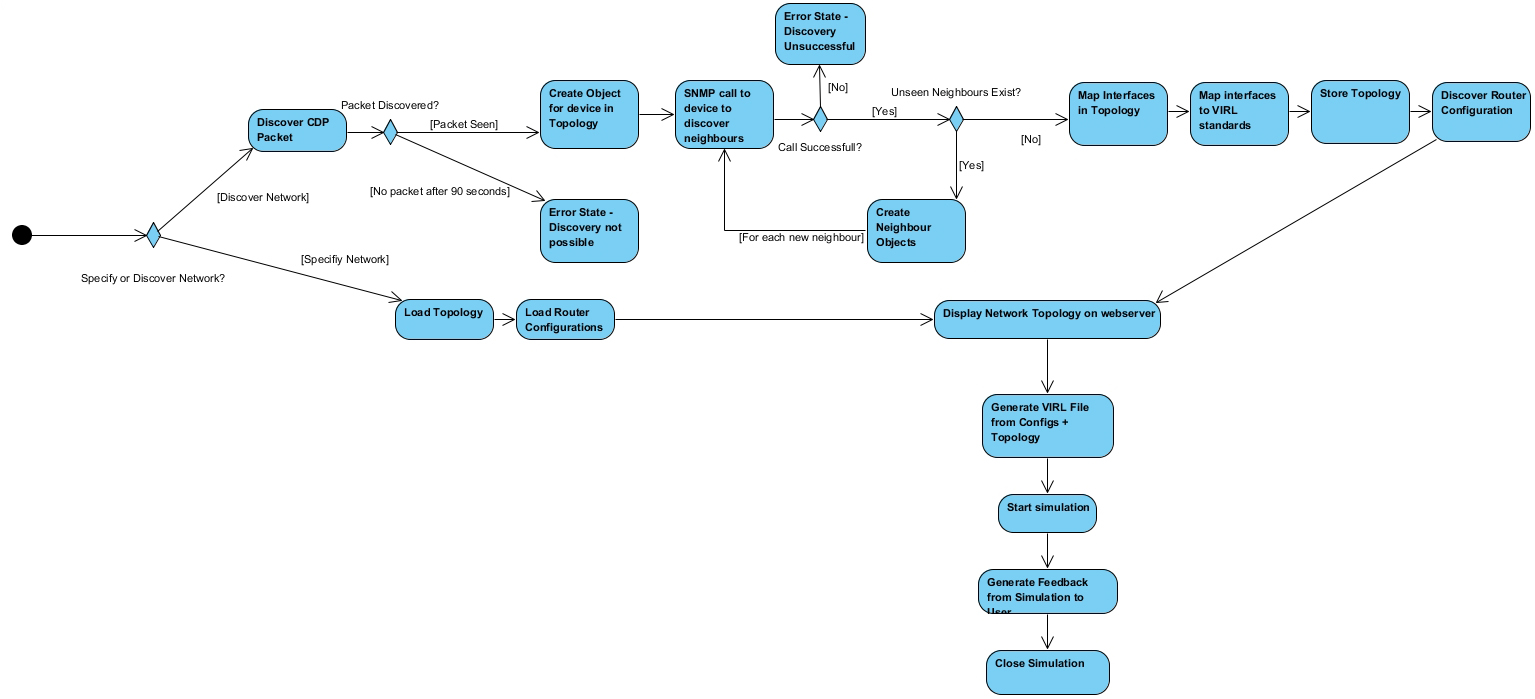
\includegraphics[width=1\textwidth]{activityDiagram.png}
\end{sidewaysfigure}

\section{Network Creation}

An emulated network can be created using two distinct inputs, the first is a copy of the configuration files for all devices in the network which will determine how the components interact with one another. For example, a configuration file can provide the settings for a routing protocol such as OSPF, specifying information required to exchange routes with other devices and choosing the networks they wish to advertise to their peers. The second input is a form of detailing the physical layout of the network, representing the devices as nodes and their inter-device links as edges. Representing this data in a format that is easily readable by a program allows the proposed tool to create emulation with all the interfaces and connections of the physical network, an accurate reproduction of these components ensures that the emulation will behave in the same way as its physical counterpart. An example of a Cisco configuration file is in Appendix E.

The proposed tool will provide two options for creating an emulated network. First allowing a user to create a version of a well-known network by allowing the input of already existing configuration backups and topology definitions from tools such as Rancid or Opsware. Alternatively, the user will be able to create an emulated version of their local network by using the tool to discover, map and backup their local devices before passing the information on to the simulation element.

\subsection{Explicit Input:}

A well-maintained network will have two components of management, the first is a detailed collection of network diagrams detailing the positions of routers and switches, the interfaces used for these links and any IP addressing these connections have. Tools used for the creation of these documents are programs such as Microsoft Visio or yED, these tools enable a Network Engineer to draw their diagrams and save them in a user-friendly visual format. A further extension of these tools allows the saving of a topology in a programmer-friendly format such as json or xml, the proposed tool will investigate using this data format for representing the emulated network. Once the topology of the network has been created it has no defined behaviour.

The second management process is a backup tool of network device configurations, large enterprise keep a backup of all router configurations as a precaution in case of unintended changes or hardware failure. If given access to these backups the proposed tool will be able to create an emulated network whose behaviour is defined by these files.

\subsection{Network Discovery}

For networks that do not have the management techniques defined above, the tool will also be able to discover devices and create an emulated version dynamically. As before, the network will require both the topology definition and the device configurations to function. In order to gather this information it will utilise some existing network technologies and standards in order to gather the information required in the most efficient method possible.

In order to map the network topology dynamically, the proposed tool will use a combination of SNMP and CDP/LLDP in order to discover the devices in the local network. These technologies, when combined will allow for the tool to create a representation of the network in an edge-and-node format which can be parsed in the emulation software. CDP is a protocol created by Cisco which details a devices local neighbours giving information such as the neighbour's hostname, device type, IP Address, the connections local port and destination port. This information can be gathered from a device by using a standard called SNMP (Simple Network Management Protocol)

Network configuration files can be extracted from running devices in multiple ways, the most common is to log on to a device and copy its configuration to a network store such as a tftp (Trivial File Transfer Protocol) server where they are stored for later use. An alternative method is through further use of SNMP to poll a device for its configuration which is returned over a terminal. The tool will use one of these methods to connect to and store a devices configuration. Once both the topology and the configuration of a network is obtained, it can then be passed to Emulation.

\section{Network Representation}

Although the VIRL system provides a topology view for running simulations, I am not intending on using this as part of the proposed tool. Instead, I will investigate methods of displaying a network using the information gathered in the Network Discovery section. I aim to investigate tools such as yED which allows the use of extensions to interact with network drawings. For example, when a topology has been drawn and displayed, it may carry additional attributes such as its IP Address, using this information the graphing software can be extended to implement features such as a terminal emulator for direct access to a device, or an API for sending defined commands to an emulated network. In addition to the interaction with the emulation, I will also investigate methods of representing feedback from devices. This information can be displayed directly on the visual topology with labels such as the status of a network connection and its current throughput. This idea can be extended and the use of colour on a network link can show the forwarding path for a destination IP address from its source. Any changes made to the routing configuration during this time will be reflected by the colour of the links and any impact of the forwarding tables for a destination can be seen.

In addition to the feedback required from a visual representation of a network, there also needs to be a level of interactivity with the network view. A topology can be viewed as its physical layout but it may have other configurations underneath this layer such as Autonomous Systems, Routing Areas or Redundancy Pairs. This information should be viewable by changing a filter on the network representation as it gives a more granular view on how the network components interact with one another. Adding these extra filters will enable a Network Engineer to view the impact of planned changes on additional aspects of the network which may not have been considered previously.

\section{Network Emulation}

The proposed tool will use Cisco's Virtual Internet Routing Lab (VIRL) as its platform for simulation, this was chosen as it provides a full Cisco IOSv image for network components which can scale more efficiently that other simulation platforms. In the proposed tool VIRL will be used as a back-end technology and the proposed tool will not make use of the Eclipse-based VM Maestro interface. The User can interact with devices by using SSH to connect to a jumphost which will provide access to the components using the management network which VIRL creates. 

In order to utilise VIRL to its fullest potential the proposed tool will connect to VIRL using its defined REST API. From initial research it is understood that a simulation can be created by creating a request to the VIRL server and including a defined .virl file. Upon receiving this file the VIRL host will create a simulation based on the on the topology defined in the file. Information about a simulation can also be obtained by making a separate request to the server for a list of running simulations. The proposed tool will make use of both of these features and allow the server to create an emulation, gather information about the emulated network and interact with the network.

\section{Interaction}

The tool will allow a user to interact with their emulated network in a variety of ways. A traditional terminal access will be provided through the web simulation as this is the primary way that an Engineer will interact with and make changes to a real network. In addition to terminal access, the tool will also investigate non-traditional methods of interaction, one benefit of producing a network diagram is the possibility of directly interacting with components in the topology, making changes such as shutting interfaces down or rebooting hardware.

Interaction with network components will provide feedback to the user through the graphical interface provided in the 'Network Representation' section. This section of the tool will display the network dynamically, using information gained from devices such as the forwarding table or bandwidth usage on a link. This information will be interpreted by the graphing software and will provide visual feedback of a network change, such as using coloured links to show a forwarding path through a network.

Connection to the emulation will be provided through a server connected to both a management network within the emulation and a public facing interface for connections from the internet. This server will facilitate the traditional command-line based connections by acting as a jumphost into the network. In addition to command-line access this server will also host a python-based web API which will allow the more unconventional methods of interaction through using networking APIs such as Cisco's OnePK tool set.

\section{Requirements}

\begin{tabular}{|l|p{12cm}|}
	\hline Requirement ID: & 1 \\ 
	\hline Description: & The system must be able to discover a physical network layout \\ 
	\hline Rationale: & A user needs to be able to discover and emulate an undocumented network \\ 
	\hline Type: & Functional \\ 
	\hline Design Constraint: & No \\ 
	\hline Fit Criteria: & A user can create an accurate model of their local network \\ 
	\hline 
\end{tabular}
\newline
\vspace*{0.5 cm}
\newline
\begin{tabular}{|l|p{12cm}|}
	\hline Requirement ID: & 2 \\ 
	\hline Description: & The system must accept existing network information \\ 
	\hline Rationale: & A user needs to be able to create a emulation based on a well-documented network \\ 
	\hline Type: & Functional \\ 
	\hline Design Constraint: & No \\ 
	\hline Fit Criteria: & A user can create an accurate model based on existing network information \\ 
	\hline 
\end{tabular} 
\newline
\vspace*{0.5 cm}
\newline
\begin{tabular}{|l|p{12cm}|}
	\hline Requirement ID: & 3 \\ 
	\hline Description: & The system will discover Cisco Devices \\ 
	\hline Rationale: & The tool needs to discover unknown Cisco devices on a network \\ 
	\hline Type: & Functional \\ 
	\hline Design Constraint: & No \\ 
	\hline Fit Criteria: & All devices on the local topology will be discovered \\ 
	\hline 
\end{tabular}
\newline
\vspace*{0.5 cm}
\newline
\begin{tabular}{|l|p{12cm}|}
	\hline Requirement ID: & 4 \\ 
	\hline Description: & The system will extract configurations from Cisco devices \\ 
	\hline Rationale: & Configuration files are required in order to emulate the behaviour of devices \\ 
	\hline Type: & Functional \\ 
	\hline Design Constraint: & No \\ 
	\hline Fit Criteria: & The configuration of each discovered device is extracted \\ 
	\hline 
\end{tabular}
\newline
\vspace*{0.5 cm}
\newline
\begin{tabular}{|l|p{12cm}|}
	\hline Requirement ID: & 5 \\ 
	\hline Description: & The system will produce a document detailing the physical layout of the network \\ 
	\hline Rationale: & A topology document will allow the tool to visually represent a network \\ 
	\hline Type: & Functional \\ 
	\hline Design Constraint: & No \\ 
	\hline Fit Criteria: & A document is produced which details the topology \\ 
	\hline 
\end{tabular}
\newline
\vspace*{0.5 cm}
\newline
\begin{tabular}{|l|p{12cm}|}
	\hline Requirement ID: & 6 \\ 
	\hline Description: & A topology map must be produced in less than 1 minute \\ 
	\hline Rationale: & Allows the discovery of a network to be efficient so it is of use to a network engineer \\ 
	\hline Type: & Non-functional \\ 
	\hline Design Constraint: & No \\ 
	\hline Fit Criteria: & Device discovery takes one minute or less \\ 
	\hline 
\end{tabular}
\newline
\vspace*{0.5 cm}
\newline
\begin{tabular}{|l|p{12cm}|}
	\hline Requirement ID: & 7 \\ 
	\hline Description: & Router configurations must be extracted in an efficient method \\ 
	\hline Rationale: & Lessens the time taken to produce a working emulation \\ 
	\hline Type: & Non-functional \\ 
	\hline Design Constraint: & No \\ 
	\hline Fit Criteria: & Configuration Extraction takes three minutes or less \\ 
	\hline 
\end{tabular}
\newline
\vspace*{0.5 cm}
\newline
\begin{tabular}{|l|p{12cm}|}
	\hline Requirement ID: & 8 \\ 
	\hline Description: & Connections to Production devices must not compromise security \\ 
	\hline Rationale: & Production devices can be left vulnerable if security is lessened \\ 
	\hline Type: & Non-functional \\ 
	\hline Design Constraint: & Yes \\ 
	\hline Fit Criteria: & The tool requires no additional access to systems when compared to an industry standard tool \\ 
	\hline 
\end{tabular}
\newline
\vspace*{0.5 cm}
\newline
\begin{tabular}{|l|p{12cm}|}
	\hline Requirement ID: & 9 \\ 
	\hline Description: & Any Cisco device can be represented within a emulation \\ 
	\hline Rationale: & A device must be able to be represented in an emulation regardless of model \\ 
	\hline Type: & Functional \\ 
	\hline Design Constraint: & No \\ 
	\hline Fit Criteria: & Any standard Cisco router will be represented in an emulation \\ 
	\hline 
\end{tabular}
\newline
\vspace*{0.5 cm}
\newline
\begin{tabular}{|l|p{12cm}|}
	\hline Requirement ID: & 10 \\ 
	\hline Description: & Network Discover will be able to cope with non-router devices \\ 
	\hline Rationale: & Not every network will be a collection solely of interconnected routers \\ 
	\hline Type: & Functional \\ 
	\hline Design Constraint: & No \\ 
	\hline Fit Criteria: & The discover will cope with Layer-2 devices such as switches and will deal with them effectively \\ 
	\hline 
\end{tabular}
\newline
\vspace*{0.5 cm}
\newline
\begin{tabular}{|l|p{12cm}|}
	\hline Requirement ID: & 11 \\ 
	\hline Description: & All interface types will be represented in an emulation \\ 
	\hline Rationale: & Cisco devices have multiple types of interfaces that need to be included \\ 
	\hline Type: & Functional \\ 
	\hline Design Constraint: & No \\ 
	\hline Fit Criteria: & Any standard Cisco interface will be represented in a emulation \\ 
	\hline 
\end{tabular}
\newline
\vspace*{0.5 cm}
\newline
\begin{tabular}{|l|p{12cm}|}
	\hline Requirement ID: & 12 \\ 
	\hline Description: & Physical interfaces will be converted into an equivalent weighting in the emulation \\ 
	\hline Rationale: & Different interface types will have different characteristics which will influence routing \\ 
	\hline Type: & Functional \\ 
	\hline Design Constraint: & No \\ 
	\hline Fit Criteria: & An interface will influence routing in the same way both in real hardware and in a emulation \\ 
	\hline 
\end{tabular}
\newline
\vspace*{0.5 cm}
\newline
\begin{tabular}{|l|p{12cm}|}
	\hline Requirement ID: & 13 \\ 
	\hline Description: & Configurations will be converted into an equivalent emulation configuration \\ 
	\hline Rationale: & The emulation must include exactly the same features and characteristics in order to be of use as a testing platform \\ 
	\hline Type: & Functional \\ 
	\hline Design Constraint: & No \\ 
	\hline Fit Criteria: & There will be no configuration loss in the emulation when compared to the real hardware \\ 
	\hline 
\end{tabular}
\newline
\vspace*{0.5 cm}
\newline
\begin{tabular}{|l|p{12cm}|}
	\hline Requirement ID: & 14 \\ 
	\hline Description: & The tool will produce a Cisco VIRL file  \\ 
	\hline Rationale: & The emulation engine, Cisco VIRL represents a topology in a VIRL file \\ 
	\hline Type: & Functional \\ 
	\hline Design Constraint: & No \\ 
	\hline Fit Criteria: & A VIRL file defining the topology is produced \\ 
	\hline 
\end{tabular}
\newline
\vspace*{0.5 cm}
\newline
\begin{tabular}{|l|p{12cm}|}
	\hline Requirement ID: & 15 \\ 
	\hline Description: & The produced emulation file will be a valid VIRL configuration file  \\ 
	\hline Rationale: & The produced file will be passed to an external process for emulation and therefore must be complete and valid \\ 
	\hline Type: & Non-Functional \\ 
	\hline Design Constraint: & Yes \\ 
	\hline Fit Criteria: & All produced VIRL files will be accepted as valid by the VIRL engine \\ 
	\hline 
\end{tabular}
\newline
\vspace*{0.5 cm}
\newline
\begin{tabular}{|l|p{12cm}|}
	\hline Requirement ID: & 16 \\ 
	\hline Description: & The tool will automatically produce a simulation when a valid VIRL file is created  \\ 
	\hline Rationale: & An emulation needs to be produced without any input by the user or any third-part GUI \\ 
	\hline Type: & Functional \\ 
	\hline Design Constraint: & No \\ 
	\hline Fit Criteria: & An emulation is created as part of the tool running  \\ 
	\hline 
\end{tabular}
\newline
\vspace*{0.5 cm}
\newline
\begin{tabular}{|l|p{12cm}|}
	\hline Requirement ID: & 17 \\ 
	\hline Description: & The emulated network will be accessible through the internet  \\ 
	\hline Rationale: & The emulation needs a method of access to the network \\ 
	\hline Type: & Functional \\ 
	\hline Design Constraint: & No \\ 
	\hline Fit Criteria: & The emulation is available online  \\ 
	\hline 
\end{tabular}
\newline
\vspace*{0.5 cm}
\newline
\begin{tabular}{|l|p{12cm}|}
	\hline Requirement ID: & 18 \\ 
	\hline Description: & The tool will provide a single server as a point of entry to the emulation  \\ 
	\hline Rationale: & Having multiple publicly available devices on the internet poses a security risk \\ 
	\hline Type: & Functional \\ 
	\hline Design Constraint: & No \\ 
	\hline Fit Criteria: & The tool provides one single publicly routable ip address for access  \\ 
	\hline 
\end{tabular}
\newline
\vspace*{0.5 cm}
\newline
\begin{tabular}{|l|p{12cm}|}
	\hline Requirement ID: & 19 \\ 
	\hline Description: & The user will be able to view a diagram of the discovered network before emulation  \\ 
	\hline Rationale: & A user will want to check the discovered network is correct before creating an emulation \\ 
	\hline Type: & Functional \\ 
	\hline Design Constraint: & No \\ 
	\hline Fit Criteria: & A diagram is produced before the network is emulated  \\ 
	\hline 
\end{tabular}
\newline
\vspace*{0.5 cm}
\newline
\begin{tabular}{|l|p{12cm}|}
	\hline Requirement ID: & 20 \\ 
	\hline Description: & The emulated network will contain a separate management network for the external server to communicate on \\ 
	\hline Rationale: & A management network will ensure that any management tools will not interfere with the emulation routing \\ 
	\hline Type: & Functional \\ 
	\hline Design Constraint: & No \\ 
	\hline Fit Criteria: & The management of the network is on an entirely separate network to the emulation  \\ 
	\hline 
\end{tabular}
\newline
\vspace*{0.5 cm}
\newline
\begin{tabular}{|l|p{12cm}|}
	\hline Requirement ID: & 21 \\ 
	\hline Description: & The user will be able to interact with an emulation in a conventional way \\ 
	\hline Rationale: & A user will want to interact with the emulation in a familiar way \\ 
	\hline Type: & Functional \\ 
	\hline Design Constraint: & No \\ 
	\hline Fit Criteria: & The user will have command-line access to any router produced in the emulation  \\ 
	\hline 
\end{tabular}
\newline
\vspace*{0.5 cm}
\newline
\begin{tabular}{|l|p{12cm}|}
	\hline Requirement ID: & 22 \\ 
	\hline Description: & The user will be able to influence the network in non conventional ways \\ 
	\hline Rationale: & The tool will provide other methods of influencing the emulated network \\ 
	\hline Type: & Functional \\ 
	\hline Design Constraint: & No \\ 
	\hline Fit Criteria: & The user will influence the network in methods other than CLI  \\ 
	\hline 
\end{tabular}
\newline
\vspace*{0.5 cm}
\newline
\begin{tabular}{|l|p{12cm}|}
	\hline Requirement ID: & 23 \\ 
	\hline Description: & The network diagram will produce visual feedback representing the current state of the network \\ 
	\hline Rationale: & The user will want to see methods other than the CLI for understanding the behaviour of the network \\ 
	\hline Type: & Functional \\ 
	\hline Design Constraint: & No \\ 
	\hline Fit Criteria: & Visual feedback is produced on the CLI  \\ 
	\hline 
\end{tabular}
\newline
\vspace*{0.5 cm}
\newline

\section{Risks}

The project has the following risks identified which could impact development:

\begin{itemize}
  \item{Constraints on access to University infrastructure}
  \begin{itemize}
    \item{External to the VIRL Server there may be a requirement to have an external server which is able to access the VIRL network - as this is in the domain of IT Services, this may not be possible}
  \end{itemize}
  \item{VIRL may not provide the functionality this project requires}
  \begin{itemize}
    \item{As the current implementation of the Cisco VIRL service is pre-release, there is some aspect of missing functionality or suffers from pre-release bugs}
  \end{itemize}
  \item{Added complexity through lack of documentation}
  \begin{itemize}
    \item{As Cisco VIRL is still pre-release and limited availability there is a lack of documentation and community support for the product}
  \end{itemize}
  \item{Requirement of Python in Cisco Development}
  \begin{itemize}
    \item{Cisco products (In particular onePK) require a knowledge of Python. This is a new language that is not well known to the developer. Therefore there may be added difficulty in understanding its function.}
  \end{itemize}
  \item{Risk of hardware failure}
  \begin{itemize}
    \item{Project may be delayed in the event of hardware failure, particularly the VIRL Server in place which requires a significant time investment to install}
  \end{itemize}
\end{itemize}

\section{Equipment Used}


\subsection{Servers}

For the production of this tool it is understood that two distinct servers are required, one local server which can handle the Network Discovery aspect of the tool and a secondary server which is contained within the VIRL emulation which will handle feedback based on changes to the emulated network. These two servers will be in contact with one-another throughout the course of a tools use. There are two solutions available for these servers, the first being a standard Linux server distribution and the second being a Windows Server installation.

One requirement of the proposed tool is the ability to display a network topology for the user to understand the layout of an emulated network. This will take form in a web browser, therefore there needs to be some aspect of a GUI on the server itself. Because of this, a standard Linux server CLI has been ruled out in favour of a more desktop-like server experience.

A second requirement of the proposed tool is the ability to interact with protocols such as CDP and SNMP. From initial research this level of interaction with packet-level networking is considerably easier and more flexible on a Unix-based operating system as existing tools can be run in a standard shell to interact with CDP. In addition to this, there are additional python libraries which can create and/or intercept packets which require a Unix operating system to run.

Due to the two requirements outlined above, it is proposed that a Linux desktop or server with display server should be used for this work. In particular, Ubuntu will be used for its user-friendliness in comparison to other distributions.

\subsection{Networking Equipment}

The proposed tool is intended to be deployed in a real-world environment, however due to the constraints I have on physical equipment for this project I have opted to create this topology in GNS3 (See ‘Existing Solutions’). GNS3 provides full simulation of IOS images and therefore is the closest representation of physical equipment. These simulations were created and run on a Windows PC using the GNS3 client. In addition to router simulation, GNS3 also has support for Virtualbox integration within the tool, this allows Virtual Servers to be connected to a topology and function correctly on a network. I will use this functionality in order to connect the Network Discovery server (as discussed in the previous section) to a separate emulated network. The use of GNS3 rather than real equipment enables a more efficient development process as work does not need to be done on-site with the physical equipment. In addition to this, the use of an emulated network allows a more thorough testing process as a multitude of testing scenarios can be created quickly, enabling more in-depth test procedures.

\subsection{Python}

In addition to physical equipment, the tool will also use Python as its primary language. This has been selected due to its flexibility and existing position in the networking development world. Due to this foothold Python has an extensive set of libraries which facilitate easier access and processing of network information.

From initial research, Python can be used to create REST network connections which allow it to interface directly with VIRL to create, edit and destroy existing simulations. Selecting Python will enable the tool to seamlessly discover networks, collate network information, create a simulation and interact with a simulation.

\subsection{CDP - Cisco Discovery Protocol}

A second software that has been identified is CDP, a proprietary protocol created by Cisco which facilitates mapping of a network through local neighbour advertisements. This protocol is enabled on all Cisco devices by default, sending an advertisement to all local neighbours every 60 seconds. In this advertisement the device specifies its hostname, whether the device is a router or a switch, the model number of the device and the interface on its local side on which it is sending the advertisement. 

From an advertisement the receiving device can piece together all the received information in order to build a picture of its local network. An example of a CDP table for a device is shown below. From this table it can be seen that there are two local routers (R2 and R3) on the local interface FastEthernet0/0. In addition to this information, it can also be seen that R2 and R3 can see R1 on their FastEthernet0/0 interfaces, with further analysis, because R1 can see R2 and R3 on the same local interface it can be inferred that there is a switch connecting all three devices.

\begin{lstlisting}
R1# show cdp neighbors
Capability Codes: R - Router, T - Trans Bridge, B - Source Route Bridge
S - Switch, H - Host, I - IGMP, r - Repeater

Device ID        Local Intrfce     Holdtme    Capability  Platform  Port ID
R2               Fas 0/0            157         R S I     3725      Fas 0/0
R3               Fas 0/0            156         R S I     3725      Fas 0/0
\end{lstlisting}

\subsection{SNMP - Simple Network Management Protocol}

An additional tool that will be used is SNMP, Simple Network Management Protocol \citep{case1989simple} is a protocol designed to allow access to sensors on a networked device. The protocol relies on a Management Information Base (MIB) which defined on a Vendor basis. Inside these MIBs there are defined Object Identifiers (OIDs) which relate to a specific sensor on the device. Access to this OIDs are managed on the device, requiring a community string which a plaintext password in SNMPv2 as a security device to prevent unauthorised access. Additional security is provided by only allowing Read-only access to OIDs which prevent malicious attacks to a system. For the purpose of this project there will only ever be a need for Read-only access, this is due to the fact that Read-Write is disabled on devices due to security concerns.

When making a call to an SNMP Agent, specifying the OID and community string the device returns a plaintext response with the requested information. This can be parsed for and adapted for use in the Network Discovery portion, or alternatively can be used in the Network Feedback sections in order to understand forwarding information. The following output shows the returned information for a call to OID `.1.3.6.1.2.1.2.2.1.2', the OID which holds information relating to the interfaces on a device.

\begin{lstlisting}
rob@netman-server:~$ snmpwalk -v 2c -c public 172.30.0.1 .1.3.6.1.2.1.2.2.1.2
IF-MIB::ifDescr.1 = STRING: FastEthernet0/0
IF-MIB::ifDescr.2 = STRING: Serial0/0
IF-MIB::ifDescr.3 = STRING: FastEthernet0/1
IF-MIB::ifDescr.4 = STRING: Serial0/1
IF-MIB::ifDescr.5 = STRING: Serial0/2
IF-MIB::ifDescr.6 = STRING: Serial0/3
IF-MIB::ifDescr.8 = STRING: Null0
IF-MIB::ifDescr.13 = STRING: Loopback0
IF-MIB::ifDescr.14 = STRING: NVI0
\end{lstlisting}

\subsection{SDN Sources using OnePK}

OnePK is Cisco's current offering on the Software Defined Networking marketplace and allows a programmatic approach to controlling and extracting information from Cisco devices.

Software Defined Networking (SDN) is a relatively new concept in the network space and although has not fully been adopted in real-world standards it can be used to extract information from routers with a relatively small footprint in production. Where traditionally a routing table of a Router would be extracted by using a tool such as a screen-scraper or SNMP, the routing table from a OnePK enable device can be requested using an API-like interface. This approach scales more efficiently than using CLI-scraping as the data can be requested through an constant connection rather than opening a telnet/SSH session. Data returned from a OnePK call can either return data in a structured format or as a copy of the text displayed on the CLI. In the case of the structured data the appropriate information can be accessed directly, in the case of screen data it can be extracted using regular expressions.

With regards to this project, OnePK will be used in the Network Feedback section in order to process information such as forwarding tables. In addition to this, it can also be used to control the network as a whole, allowing the tool to make changes to interface states or costs in order to influence routing decisions.

\chapter{Implementation}

\section{Lab Design:}

\begin{figure}[h!]
\caption{GNS3 Topology}
\centering
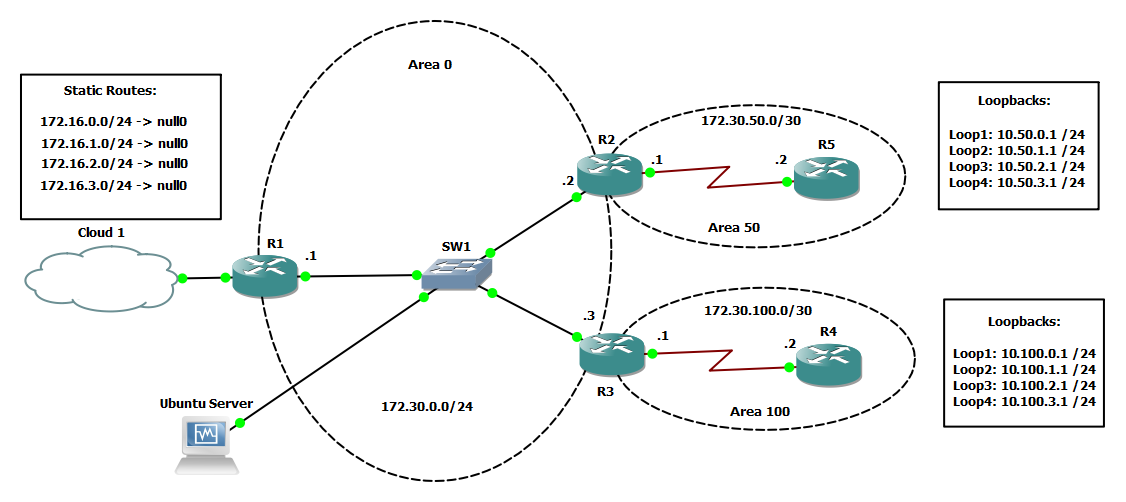
\includegraphics[width=0.8\textwidth]{Lab-Design.png}
\end{figure}

A key feature of the simulation tool is the ability to replicate a 'Real-world' network in emulated space. In order to gather the information required for this feature an extra tool set for Network Discovery has been created. This allows a user to discover devices on the network and extract interface information and router configurations in order to build an emulated instance of the network.

For the development of this Router Discovery tool the above topology was created and used. As explained earlier this is implemented within GNS3 to utilise its simulation of real IOS images. The above shows a Topology I have created as a use-case for emulation testing, an Ubuntu 14.04 server is also attached to the topology will which be used for the Network Discovery portion of the tool. In addition to this server, a `cloud' object is also connected, this provides internet access to the Lab through a bridged interface on the local machine.

The Ubuntu server is implemented using VirtualBox integration within GNS3 and allows direct connection to the 172.30.0.0/24 network. This Ubuntu server will hold the tool used for Router Discovery and Configuration Extraction. As this server is sitting on the same private network as all of the routers this allows me to find all the routers using defined ip addresses or through using CDP.

The connection to the Internet is provided through the cloud in the diagram above. This is inbuilt functionality within GNS3 which allows the topology to interface with the local host’s connection. This is implemented by adding a loopback to the local PC and bridging the internet connection to this loopback. GNS3 then connects to this loopback address and provides an interface to the Internet in the form of the Cloud object. Once this connectivity is provided the topology has a defined router which is used for internet connections, in this scenario R1 provides the connection. This router is then configured to provide dhcp to any servers on the local subnet, providing a default gateway and DNS Servers for the connected hosts. This router is also configured to provide NAT services in order to allow these private addresses to communicate to the outside world. Once internet connectivity is established the system can deploy.

The base lab used for development has been designed to contain different elements of networks that may be faced in a real-world scenario. The routing of the network is provided via OPSF, a Distance Vector protocol which is used for interior routing in large enterprise. The network is broken into four OSPF areas, these segment the network and prevent routing tables from becoming too large. A second characteristic of this lab is its inclusion of switches, these are `dumb' switches provided by GNS3 and are not running the Cisco IOS, however they introduce additional complexity to the network which the tool will need to deal with efficiently. The final characteristic of the network is the types of interfaces. As seen in Figure 5.1 the topology includes two distinct types, the first is the expected FastEthernet interfaces which is used for the majority of modern connections, the second is a more traditional Serial interface which would be used for long distance leased-line connections. The variety of interfaces will need to be included in the emulation and their behaviour will also need to be reproduced as it will influence routing decisions.

\section{Network Documentation}

One key feature of the documentation of a network is the data structure that will define it. As discussed in the design sections, a network can be defined with two documents, the device configurations and the physical layout of the connections. The tool provides the latter through a python object referred to in the code as 'topology' is of class routerList. At its highest level this object is a list of the devices that are on the network, this code for the class is shown below:

\begin{python}
	class routerList(object):
		def __init__(self, routerList):
			self.routerList = []
	
		def addRouter(self, routerEntry):
			self.routerList.append(routerEntry)
	
	class router(object):
		def __init__(self, cdp_entries):
			self.cdp_entries = []
			self.hostname = ''
			self.ipAddress = ''
			self.capabilities = ''
	
		def addCdpEntry(self, cdp_entry):
			self.cdp_entries.append(cdp_entry)
	
		def addHostname(self, hostname):
			self.hostname = hostname
	
		def addIpAddress(self, ipAddress):
			self.ipAddress = ipAddress
	
		def addCapability(self, capability):
			self.capabilities = capability
	
		def removeCDPEntry(self, interfaceName):
			#Updates cdp_entries to include only those that DO NOT match interfaceName
			self.cdp_entries = [cdpEntry for cdpEntry in self.cdp_entries if cdpEntry.srcPort != interfaceName]
\end{python}

As seen above, routerList is a list of all devices on the network. At a lower level, a router is any device found on the topology, it is comprised of a Hostname, IP Address, capabilities and a list of CDP entries for the device. CDP Entries are used to define the physical connection on the topology and when fully processed each interface will have a single CDP entry per interface. A more detailed view of a CDP entry is as follows:

\begin{python}
		class cdpEntry(object):
			def __init__(self, hostname):
				self.hostname = ''
				self.srcPort = ''
				self.dstPort = ''
				self.ipAddress = ''
		
			def addHostname(self, hostname):
				self.hostname = hostname
			def addIpAddress(self, ipAddress):
				self.ipAddress = ipAddress
			def addSrcPort(self, srcPort):
				self.srcPort = srcPort
			def addDstPort(self, dstPort):
				self.dstPort = dstPort
\end{python}

As shown above, a CDP entry comprises of a Hostname, IP Address and source and destination ports. This information maps the links in the topology. In this instance, the Hostname and IP Address relate to the remote device on the link. This information allows the routerList object to hold the full physical layout of the topology.

\subsection{Network Discovery}

Network Discovery allows the user to dynamically understand the topology of local network. The user has additional options available when taking this route to simulation. If the user specifies the --specify option when running the script, the tool will present them with an interactive prompt where the user can specify the network ranges to be added to the simulation. This is shown below:

\begin{lstlisting}
root@netman-server:~/NetworkSimulation/python-scripts# python NetworkDiscovery.py --specify
Enter the network address at the first prompt, followed by the subnet at the second. Type "end" to finish
Enter the network address:
172.30.0.0
Enter the subnet mask in CIDR notation (Example: /24)
/24
Enter the network address:
192.168.0.0 
Enter the subnet mask in CIDR notation (Example: /24)
/16
Enter the network address:
end
\end{lstlisting}

This functionality uses a module called ipaddr \citep{ipaddr} which creates an object bound to the IPv4 specification, this enables the tool to check user input for erroneous entries such as entering an IP address rather than a network. Setting the tool to run with specified networks sets a flag which is used throughout the tool's operation to ensure that discovered devices are within the bounds of the networks identified.

As this tool focuses on the emulation of Cisco devices it allows the tool to utilise Cisco standard technologies as a method of interacting with devices. One such technology is Cisco Discovery Protocol (see 4.8.4) which is a protocol enabled on all Cisco devices allowing them to understand the local network. This protocol is sent as a broadcast on the device's local network, the tool takes advantage of this fact as it can `sniff' for a CDP packet in order to discover the closest Cisco Router. To do this, the tool uses an external program called Cisco Discovery Protocol Reporter (CDPR)  \citep{CDPR} to listen on a local interface for a CDP Packet. Once a packet is seen, CDPR returns hostname and IP Address of the device that created the packet.

This function is defined in Appendix A, it uses a python library called os, this allows the code to create a subprocess on the server in order to run external programs. This subprocess runs CDPR on the eth0 interface and then returns the output from the subprocesses pipe, at which point python saves this to a variable and processes this variable until only the Hostname, IP Address and capabilities of the device remain. Once this information is extracted the tool creates a base router, this is used as a starting point of the Network Discovery process.

Error handling occurs in this function through the use of a timeout in CDPR. The default send time for a CDP process on a Cisco device is 60 seconds so it can be assumed that if not packet is received after 61 seconds there is no local Cisco device on the network, when this error is hit the tool notifies the user and then closes the script entirely as no further processing can be done.

One caveat of using CDPR as a tool is its requirement of root privileges in order to look at network traffic, because of this the this portion of the tool requires superuser access. on the host. One alternative to this was to write the code with an expect module, which would allow the current account to request root privileges. However this would require the script to know the local user's password, this is insecure and was deemed too much of a security risk.

Once a baseRouter is created, this object is used as a point of entry into the network. The tool then runs a series of SNMP calls to the device looking for CDP information such as hostnames, IP Addresses and interfaces. These functions make calls to the device specifying the OID the information it requires. The OIDs used in the code are defined in Figure 5.2.

\begin{figure}[h!]
	\caption{OID Definitions}
	\centering
	\begin{tabular}{|l|p{11cm}|}
		\hline \textbf{Object Identifier} & \textbf{Description} \\ 
		\hline .1.3.6.1.4.1.9.9.23.1.2.1.1.6 & Returns a list of Hostnames which are sourced from CDP \\ 
		\hline .1.3.6.1.2.1.4.1 & Returns the value of the device's forwarding (Layer 3 routing) setting, this is used to determine whether a device is a switch or not \\ 
		\hline .1.3.6.1.4.1.9.9.23.1.2.1.1.4 & Returns a list of IP Addresses which are sourced from CDP \\ 
		\hline .1.3.6.1.4.1.9.9.23.1.2.1.1.7 & Returns a list of remote interfaces which are sourced from CDP \\
		\hline .1.3.6.1.2.1.2.2.1.2 & Returns a list of local interfaces on the device \\
		\hline 
	\end{tabular} 
\end{figure}

The SNMP interaction consists of one function per SNMP call, in this function the call is made, the data is processed and a list of information related to the call is returned. a pseudo code version of this function is shown below:

\begin{lstlisting}
function getCDPHostnames(router):
	Make an SNMP call for hostnames seen in device's CDP table
	Store the returned data into a variable
	Parse the output until only the hostnames remain
	Return a list of hostnames
\end{lstlisting}

This information is added to the baseRouter object, at this point in the code only the base router and its links are known. At this point a recursive function updateRouters is called. This recursive funtion discovers all remaining devices in the topology. The control for this function is based on whether routers that are currently seen already exist in the topology object, if already known, the routers are ignored. Alternatively, if the routers are unknown an object is created for them and the function is recursively called with the new routers. The below pseudo code gives shows the logic used in this recursive discovery, the full implementation can be seen in Appendix B.
\pagebreak
\begin{lstlisting}
function updateRouters(updateRouter, topology)
	Get all hosts connected to updateRouter
	Get all IP Addresses connected to updateRouter
	FOR each host identified
		IF a router does not exist for this host
			Create a new router for this hostname
			Get hostnames connected to the new device
			Get IP Addresses connected to the new device
			FOR each device connected to the new device
				Create CDP Object for each connection on the new device
				Add CDP Object to the new device
			Add the new device to the Topology
			Call updateRouters with the new device
\end{lstlisting}

The function has two distinct paths, it can either add all devices it discovers to the topology. In this case the code following line 52 is executed, a device is added to the topology if it is unknown. An alternative path is the on line 13, the checkNetworks flag is set to true, all devices are checked against the list of required networks and if any do not match they are ignored. This method is effective for removing unwanted devices from the topology, however the connection from other devices to the device in question will still remain. Any links that do not have a defined destination will not create a valid JSON or VIRL file and the emulation engine will fail. In order to avoid this situation, when an unwanted router is encountered it is logged to a global variable, unresponsiveDevices after device discovery is complete a function removeUnresponsive() deletes any links with reference to these devices from the topology. Pseudo code for this function is shown below:

\begin{lstlisting}
fuction removeUnresponsive(topology):
	Create a set of unresponsive devices
	FOR every unresponsive device:
		FOR every device in the topology
			FOR every cdp entry in this device (links)
				If the link connects to the unresponsve device, remove it from the topology
\end{lstlisting}

Once the unresponsive devices are removed from the topology the first stage of the emulation layout is complete, however in its current form the topology will be rejected by VIRL. This is because VIRL only supports GigabitEthernet interfaces in an emulation, the topology needs to be reformatted to remove any FastEthernet or Serial connections and replace them. This is handled by formatInterfaces(). The function looks at each device in the topology, inspecting each interface on the device and mapping the interface to a GigabitEthernet connection on the emulation. It maintains a list (intChanges) of each host and the interfaces that were changed on the host, saving them to a file for use in the configFormatter section of the tool.

When the function is nearing its end it passes this list on to the replaceInterfaces() function. This function iterates intChanges, looking at every device in the topology and each CDP entry for that device. When the function meets the current device in intChanges it looks for any CDP entries that have a source interface of the interface to be changed, once it is found the interface name is replaced with its emulated counterpart. At this stage in the discovery process there can be multiple CDP entries with the same source interface, this occurs when there is a switch in the network. When designing this function this caused issues as there can be an expectation that CDP entries map to interfaces in a one-to-one fashion, in the original version of this function a flag was set when a source interface was changed. However, this was naive as when this code was deployed to topologies that were not just point-to-point links the code would fail as pre-emulation interfaces would remain after the function ended.

\begin{lstlisting}
function replaceInterfaces(topology, intChanges):
	FOR each change entry
		FOR every device on the topology
			FOR each device's CDP entries
				IF the device is the one to be changed and this is the port to be changed
					Update the port
				IF the device is not the one to be changed but has a connection to the device in question
					Update the remote port in the CDP entry
	
\end{lstlisting}

One important aspect of this function is ensuring that CDP entries of devices that connect to the device in intChanges are also updated, the second statement in the function allows for this and checks the CDP entry on every device, if the device has a CDP entry connecting to the current device to be updated the destination port is updated. Doing this ensures that all links in the emulation connect to the correct location.

At this point in the Network Discovery process the physical layout of the topology is known, however there is additional information that can be extracted from the topology, one example is the identification of Layer-2 devices such as switches. One indication of such device is a router including two CDP entries on one interface, this shows that there are two local devices connected through one physical cable which is not possible without some layer-2 device in the middle. To accommodate switches the tool has a function findSwitches() which is documented in Appendix C. This function again iterates over all the devices in the topology, for each device it notes the occurrence of each local interface in the CDP entries. If any encountered interface already exists in the seen set it is noted as a duplicate and added to the dupes list.

The function then inspects this dupes list (if any duplicates exist) for each duplicate a switch is created for the LAN segment connected to the interface. This switch is given a hostname and CDP entries are created both for the local interface and for the remote interfaces that are connected to the local link. This effectively splits the connection in half, inserting a switch into the link which connects to both routers. Once the switch is created, another function updateSwitchLinks() is called which will update the CDP entries on the local and destination interfaces.

The function updateSwitchLinks() iterates through each update, looking at each host's CDP entries until the defined in the update is seen. At this point the function replaces the remote devices CDP information with the new entries generated for the connections to the switch. At this the topology is complete and ready to be passed to the next stage.

The second stage of the discovery process is configuration extraction from the devices defined in the topology. For reasons explained at the end of this section, an external tool called Rancid \citep{Rancid} was used for this section of discovery. The configuration extraction is defined in the file rancidSetup.py, in this script the router dictionary produced by networkDiscovery is used to create a group of devices in rancid's configuration. Once a group is created and defined the script logs in as the rancid user on the host. Once logged in the rancid user runs the script rancid-cvs, this script creates a CVS repository for the group that has been created. The user then adds the configuration for the routers, first adding each hostname to router.db within the group which adds the router to the extraction process. After adding this it then adds the login information for each router to rancid's .cloginrc file. This file defines the method of connection, which is ssh with 3DES encryption for this script. It also adds the login credentials which must be configured on the router. Once this information is saved the script rancid-run is called, this starts the configuration extraction process.

While creating this section of the code it was difficult to produce a method that did not breach Requirement 8 in the Requirements section (4.8). This requirement relates to security methods of interacting with a Router on a Production network and requiring this tool to not introduce security flaws in these networks. In initial designs the tool would extract configurations itself using SNMP to poll each router, however when reading around this subject it became clear that this method of interaction with the routers would require Read/Write access on SNMP. This access was defined on a device level and not to a single OID, and thus would leave any devices exposed to exploitation if this access was mismanaged. Due to this the decision was taken to offload this section to a standard tool in the Networks world. Rancid was chosen due to its lightweight design and licensing which allows its use without any additional purchases or fees.

One issues faced when implementing RANCID on my lab network was that by default Cisco routers are set to SSH Version 2, this requires additional configuration on the device such as a domain and generation of an RSA key for access. For the design and testing phase of this development this expectation was removed through the use of `ip ssh version 1' on each device. However in normal operation SSH will be set up on each device and this error will not occur.

\subsection{Network Entry}

Network Entry works in a similar fashion to Network Discovery, however the devices on the emulation are created by reading a json file documenting the physical layout of the topology and also adding the configuration files for each device in the 'config-files' directory in the script's location. The script first loads the topology json file, creating a new router object for each node defined and adding it to the overall topology. The second operation loads the link information from the json, however this needs to mapped to CDP entries in order to follow the networkDiscovery convention. To do this the sourceRouter for each link is read and then mapped to the correct device in the topology. This creates a full network.

At this point the topology file is ready to have its interfaces mapped to emulated  as was the case in networkDiscovery. The topology is passed through the same formatInterfaces function as before and interfaces are mapped to their emulated counterparts. The same routerDictionary and interfaceChanges lists are created and saved to a file. From this point forward both the discovered and input networks are treated in the same way. 

\section{Configuration Editing}

Before creating a simulation the Cisco configuration files need to be edited in order to match the new layout defined in the topology files. Specifically the interfaces need to be replaced with their emulated versions and an additional interface needs to be added for the management network when the emulation is live. Due to the fact that a Cisco configuration file is based on a hierarchy to edit the file directly as changing information under an interface could break the hierarchical link between the interface and its children. In order to overcome this issue, the tool uses an additional python library, ciscoconfparse \citep{ciscoconfparse}. This library allows python to read a configuration file and break it down into the relevant parent-child relationships that are required to make a clean edit to the interface.

The extraction of the parent-child relationships in a configuration file allows the tool to make changes to interfaces without any loss in configuration. For example, an interface that has been set to passive in a routing protocol would need to be reflected in an emulation. Removal of a passive interface could introduce errors into an emulation as this interface can now negotiate routing with the devices it connects to, this could have impact of the routing decisions made on the topology. Maintaining this mirrored configuration ensures that the emulation generated for a network is a as true to real hardware as possible.

An additional feature that was considered was the type of interface before it is converted to an emulation Gigabit interface. When representing a FastEthernet interface on an emulated network it replacing the port in name-only would be representing a link with a maximum bandwidth of 100mb/s with one that is 1000mb/s. This direct replacement would break the routing decisions as all links on the topology would become an equal weighting. In order to prevent this the tool appends a child to each interface relating to the original bandwidth of the link, for an interface that was originally FastEthernet a `bandwidth 100000' child is added to the interface. If an interface was originally a serial connection, a `bandwidth 2000' child is added, this is the speed of an E1 connection. If any such configuration exists under the interface it remains and no action is taken.

After the relevant changes are made to interfaces on the configuration, a new interface is added. Within VIRL there the ability to connect the topology through a management network, this as called a Private Simulation Network. In order to allow this network to function an additional interface, GigabitEthernet0/0 is added to each configuration file.

Finally any information pertaining to security on the device is removed from the configuration. This is to allow access to the device when it is on the emulation. Information such as the the login credentials and enable password are removed, in addition to this the vty lines on the device or opened with the `no login' command.

\section{VIRL File Creation}

As discussed in Section 4.4 an emulation in Cisco VIRL is defined through an xml-based file known as a virl file. In order the data gathered up to this point to be represented in a valid virl format the tool uses an external library called lxml \citep{lxml} to create xml tags based on the topology. This allows the tool to quickly generate correct xml that the VIRL host recognises as valid.

This section of the tool is outlined in the file virlCreation.py. In this file the tags are first created to hold the xml and virl specifications which are then added to the xml object. After this, the script adds information to the topology as a whole, such as specifying that CDP is enabled and that the devices are running the onePK API. One key feature that is added at this point is is setting for a management network on the emulation, setting this to `exclusive' specifies that the management network is local to the emulation and does not interact with other simulations.

Once the settings are defined the script then loads the routerDictionary which was defined earlier in the tool. It then begins to iterate over each device, creating a node tag for each and setting the device to an IOSv Router for any routers seen or to a SEGMENT for any switches seen.

One issue encountered when designing this section of the tool was finding a way to efficiently represent a switch on the network. Losing the connectivity provided by a switch would introduce extra links to the topology that will in turn create discrepancies between the emulated routing and the real hardware routing. Due to this fact, the tool uses the device SEGMENT. This device produces a layer-2 broadcast domain which acts in a similar fashion to the switch. In later versions of the VIRL software these segments have been replaced with `dumb' switches. These act in a similar fashion and do not make real switching decisions, however a full IOSvL2 image is due to be added in the next version of Cisco VIRL.

Once the node is created for a device the configuration is then added, to do this the script loads the router's `.edited' configuration file that has been produced in the local `config-files' directory. This configuration was produced in the previous section. The tool appends the contents of this file to the nodes `config` attribute. Once the configuration has been added the tool then iterates of the routers CDP values, adding an interface for each one. At this point the CDP Values give unique interfaces as switches have been added to the topology. This interface does not dictate the physical links in the topology.

An additional entry at this point is made to the emulated topology. This is an ubuntu server which will act as a gateway into the network. This implementation uses two distinct objects in the virl file. The first is the server, this is created using a cloud-init script defined in Appendix F. This sets up basic access on the server such as user accounts and home directories. An interface is added to the server for its connection to the internet. The second object is a SNAT Object, this provides Network Address Translation between the emulation and the outside world, when configured this object allows inbound connections to the server.

The final part of this file defines the connections between the devices in the topology. This section proved difficult as the design for a VIRL file does not match the design that has been used for the storage of information up to this point in the design. The links in a VIRL file are mapped using the relative position of the devices in the file rather than the identifier that has been assigned, in addition to this there is only one definition of a link regardless of the source and destination device. This introduced additional complexity to generation of the virl file. This was overcome by adding an additional check against a list of existing interfaces on the topology file.

Once all devices and links have been added to the xml object the file is generated and saved locally as the file `topology.virl'

\section{Simulation}

At this stage of the implementation an additional barrier to the design was introduced. The VIRL host that is used for all simulations is only contactable if the host machine is connected to the Loughborough University VPN. This added a requirement that the tool must be run on the VPN in order to be granted the appropriate access. A second requirement was that the local host machine must have a shared interface in order for the Lab design in Section 5.1 to connect to the Internet. It is now understood that a security requirement on the Loughborough VPN and Eduroam network dictates that any devices with a shared network interface is blocked from connecting, this created a conflict in the design.

In order to overcome this issue, the design now uses two identical servers with differing network connections in order to create a simulation. In this design the server on the lab network gathers and collates the information about the network, produces a virl file and then uploads this file to an intermediate SFTP server. Once this has been uploaded the lab is powered down and the same server is loaded, however this instance uses a traditional NAT connection to the internet. This allows it access to Loughborough University infrastructure and the internet. This server downloads the VIRL file from the SFTP server and pushes it to VIRL to create an emulation.

The simulation aspect is handled in the file uploadTopology.py. This file connects to the Cisco VIRL REST API in order to create and retrieve information about simulations. The script begins by loading the virl file into a variable, it then creates a POST request to the API's `/simengine/rest/launch' rule. In this request it attaches the virl file and a defined naming scheme to be included in the simulation ID. The server then makes a GET request to the API's `/roster/rest/' rule, this returns information for every node on every simulation for the user that is authenticated. The script iterates over this information, for every IOSv need it sees for the simulation made it keeps a dictionary of the IP Address and hostname. When the function meets the `virl-sim-server' for the current simulation it saves information such as it's internal address, external address and the port number for which a user can access the server's console line.

\begin{lstlisting}[caption=Extract of /roster/rest information]

"rob.My_Topologies@topology-gymofc.virl.~lxc-flat.External Address": {
"Annotation": "131.231.97.151",
"SimulationHost": "158.125.102.75",
"managementIP": "131.231.97.151",
"simExpires": null,
"simID": "My_Topologies@topology-gymofc",
"simLaunch": "2015-01-06T16:06:59.534563",
"simStatus": "ACTIVE"
},
"rob.My_Topologies@topology-gymofc.virl.~lxc-flat.External Port": {
"Annotation": "59313",
"SimulationHost": "158.125.102.75",
"managementIP": "59313",
"simExpires": null,
"simID": "My_Topologies@topology-gymofc",
"simLaunch": "2015-01-06T16:06:59.534563",
"simStatus": "ACTIVE"
},

\end{lstlisting}

The information gathered about the IOSv hosts and the virl-sim-server are used in the function setupServer(). At this stage in the simulation the server does not have a valid network configuration. This function uses a telnet library, telnetlib \citep{telnetlib}. Telnet was used for this section of development as the only internet-facing access into virl-sim-server is a console port provided on VIRL. The function telnets into this console port, gaining access to the console line. The tool then configures the eth1 IP address to match the internal SNAT address that was received earlier in the function. At this point the server has a valid IP address and can communicate with the outside world, however it does not have a default gateway so cannot respond to traffic. The function adds this default gateway to the server's routing table. The server can now contact with the outside world, the tool returns the IP address of the public-facing interface and the user can SSH into the virl-sim-server, using it as a jumphost into the simulation.

\begin{figure}[h!]
	\caption{Management Network Design}
	\centering
	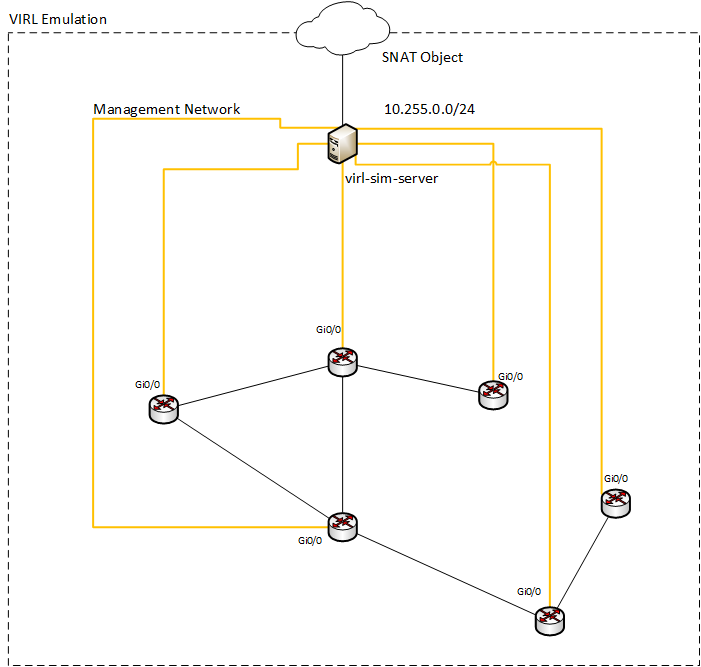
\includegraphics[width=0.7\textwidth]{managementNet.png}
\end{figure}

Figure 5.3 shows a simplified view of the network produce in VIRL. In this diagram the emulated routers are represented by the router icons and `real-world' cables are represented by black links. In addition to these links the emulation also has a management network, denoted by the yellow links, which interconnects every device on the network. For simplicity, Figure 5.3 only shows the management connections through to the virl-sim-server, this network operates on the 10.255.0.0/24 subnet. All IOSv on the topology connect via the GigabitEthernet0/0 interface created in Section 5.3. This connectivity will be used to allow the virl-sim-server to connect and gather information from the IOSv devices on the topology.

\section{Interaction}

The produced tool allows a Network Engineer to SSH to the virl-sim-server, from here the user can interact with the emulation through a traditional method, telnet. This provides unrestricted access to the device's VTY lines from which an engineer can implement any changes to the network, gathering feedback via methods such as viewing routing tables or looking at traceroutes through the network. In addition to the VTY access an engineer can also deploy other tools on to the virl-sim-server which can connect to the emulated routers. Examples of these tools are outlined in the following subsections.

\subsection{SNMP Monitoring}

IOSv instances, the focus of this tool support SNMP just as a physical router would. Using this access I can set up an SNMP Monitor on a server within the simulation which could provide detailed statistics such as interface counters. Using this information the system can determine at a high-level where traffic is flowing.

\subsection{Netflow}

Cisco Flexible Netflow is supported by Cisco IOSv and gives a more detailed view of traffic across router interfaces. Configuring each IOSv instance as a Flow Exporter and adding an collector such as Cacti will provide a detailed breakdown of traffic based on its Layer 3 and 4 information. This adds further granularity to the testing evidence that is created.

\subsection{Packet Capture}

All interfaces within VIRL have a defined 'tap' interface on the VIRL Server, this can be used for packet captures. Using a packet capture in addition to the Netflow and SNMP will allow the tool to inspect the traffic at a much more granular level. One use case of this would be the testing of a routing change on an established session and how an application can deal with this.

\textit{Note: Access to these tap interfaces may require access to the VIRL server in the admin role}

Although this adds value to the tool produced, it unfortunately does not meet the full requirements outlined in the  

\chapter{Testing}

To support the development of this project I have created a set of network topologies with complex configurations. These are a representation of a network which a user may wish to simulate and can demonstrate added complexities which may be encountered in a real-world networks. In addition to this, they provide an already established routing platform which can be used for testing network changes. As described in the previous section "Equipment Used" these topologies have been created inside of GNS3.

\section{Topology 1: Multi-area OSPF}

\begin{center}
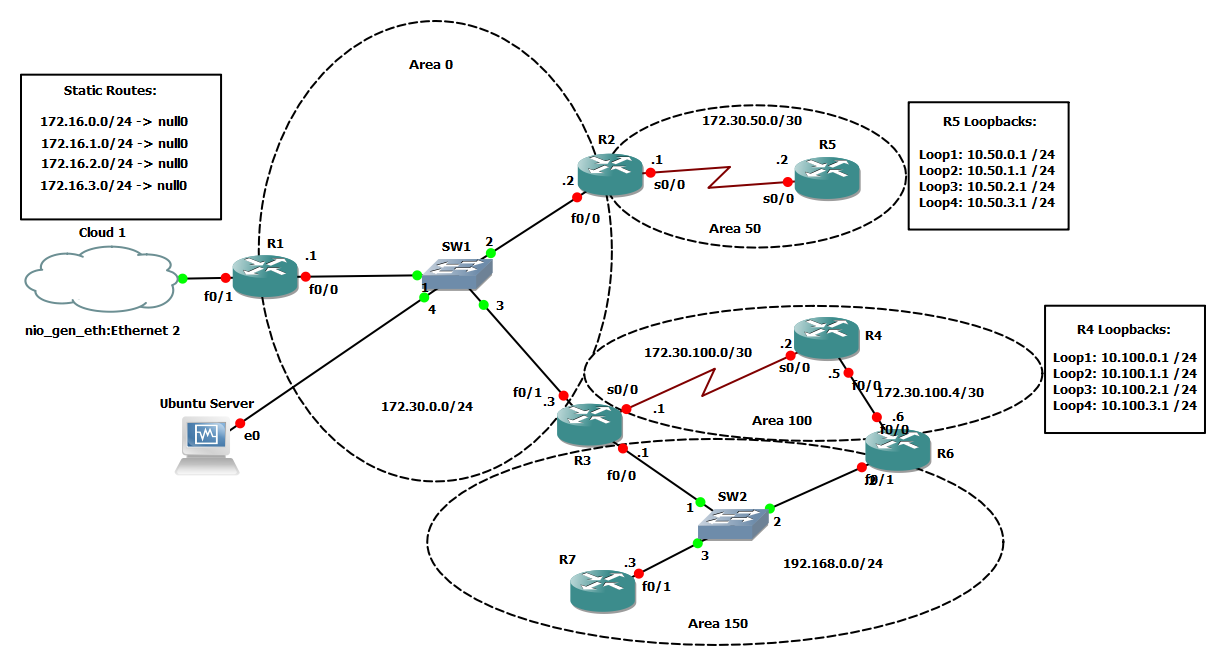
\includegraphics[width=0.8\textwidth]{OSPF-Topology.png}
\end{center}

I have designed this Topology to represent a simple network with a complex OSPF routing set-up, which may be a possible scenario that a network engineer may wish to experiment with before implementing changes in Production.

The topology represents the OSPF backbone of a large enterprise network, it includes three OSPF areas; area 0 (Backbone), area 50 and area 100. In this scenario R2 and R3 are taking the role of Area Border Routers (ABR) and providing route summarisation between the areas. For both area 50 and area 100 there are also addition Loopbacks created on the end routers which provide additional routes for this summary.

In addition to the routes being introduced via the loopbacks on R4 and R5 the topology also injects external routes into OSPF on R1. These are static routes defined on R1 which represent routes from either the Internet or routes from another routing protocol such as EIGRP, IS-IS or BGP. In this form the routes are sent to null 0 (blackhole) as there is no need for connectivity to them.

\section{Topology 2: EIGRP Based Routing}

\section{Topology 3: Service Provider BGP Topology}

\chapter*{Implementation Notes}

\section*{Simulation Tools}

\subsection*{Simulation Start}

A simulation can be started on the VIRL host itself by specifying the .virl file to be processed and the user workspace for it to be used in. This process is shown below:

\begin{lstlisting}
virl_std_client simengine-launch --virl-file /path/to/starter.virl
Session ID is starter-Ewn0Mn
export STD_SESSION=starter-Ewn0Mn
\end{lstlisting}

\subsection*{REST API}

Details of the current running simulations for an account can be determined via the following URL: http://virl.lboro.ac.uk:19399/roster/rest/

The output of this called is shown in section 4.3

By analysing the output of this data the public ip address of the LXC Host can be determined and access to the simulation can be granted.

\subsection*{LXC Host}

The LXC host is created when the simulation is first started, by selecting the Management Network type as a 'Private Simulation Network'. Upon the start of a simulation an additional Linux Container (LXC) will be created. This container will be available on a public ip address and can be accessed externally (within the Loughborough network)through SSH. Once connected to the container all other hosts on the network are directly connected and can be accessed using their management ip address.

\section*{Connectivity Tools}

\section*{Creation of SNAT Connection}

As described in the LXC Host section, all hosts can be accessed externally by using the LXC host as a jumphost into the simulation. However, this does not provide routing to the outside world. A use-case for the SNAT object would be a single point of exit to the outside world, as would be used in a standard network infrastructure. Connecting a SNAT object to a designated 'external' router can provide access to the entire simulation if required.

\subsection*{Default Routes}

For any devices that require a SNAT object, a route needs to be added on the router for connection to the SNAT object. This can take the form of a default route (below)

\begin{lstlisting}
ip route 0.0.0.0 0.0.0.0 10.254.0.1
\end{lstlisting}

\subsection*{Server IP Addressing}

When connected to a multipoint connection a server is assigned an ip address in the subnet range, this is usually done sequentially. Alternatively this can be defined in the .virl file.

\subsection*{Server DNS}

DNS Servers can be added to a host by editing the /etc/resolv.conf file. Alternatively they can be provided to a server if DHCP is enabled on the router.

\section*{RANCID Installation \& Use}

Look to set up SSH rather than telnet (For security)
\\
Change Protocol type on router side (2vs1)
\\
NOTE: Hostnames in the .cloginrc file need to be lowercase

\section*{Initial Discovery}

Use cdpr on the discovery server in order to discover the default gateway address + port

sudo apt-get install cdpr

sudo cdpr

\section*{Python Path}

 export PYTHONPATH=/opt/cisco/onep/lib/python2.7/site-packages
 
\section*{SNMP to get CDP Neighbors}

snmpwalk -v 2c -c public 172.30.0.1 .1.3.6.1.4.1.9.9.23.1.2.1.1.6.1.2

.1.3.6.1.4.1.9.9.23.1.2.1.1 - Gives information of sh cdp neigh

1.3.6.1.4.1.9.9.23.1.2.1.1.6  - Gives the hostnames of CDP neighbours 

.1.3.1.4.1.9.9.23.1.2.1.1.4 - Gets the ips for the above

.1.3.6.1.4.1.9.9.23.1.2.1.1.7 - Gives local interfaces

.1.3.6.1.2.1.4.1 - Gives ip forwarding (1 is router, 0 is a switch)

.1.3.6.1.4.1.9.9.23.1.2.1.1.7 - Gives interfaces on neighbour

\section{Virl Server Setup}
route add default gw 192.168.1.254 eth0

\section{Change server interface ip}
ifconfig eth1 up 10.254.0.36 netmask 255.255.255.0

\bibliographystyle{plainnat}
\bibliography{bibliography}

\begin{appendices}

\chapter{Function getLocalCDPInfo()}
\begin{python}
def getLocalCDPInfo(baseRouter):
	#Function listens on interface for a CDP packet and creates a router if successful. Script closes if no packet found
	try: #Catches exception generated when CDPR returns null (CDP packet not seen)
		cdpdiscovery = subprocess.check_output(["cdpr", "-d", "eth0", "-t", "61"])
		#Starts subprocess for CDP, timeout is set to 61 as default CDP timer is 60
		#CDP returns the information in lines, below code breaks in into a list and processes the information 
		cdpList = string.split(cdpdiscovery,'\n')
		cdpValues = [s for s in cdpList if re.search('value', s)]
		for idx, val in enumerate(cdpValues):
			cdpValues[idx] = val.replace(" ", "")
		for idx, val in enumerate(cdpValues):
			cdpValues[idx] = val.partition(':')[2]
		#The below code creates a router object for the baserouter and returns it to main
		if checkNetworks == True:
			#Networks ranges have been specified for discovery
			notInNetwork = True
			ipAddress = str(cdpValues[1]) + '/32'
			#Create string to hold device IP address
			for idx, val in enumerate(specifiedNetworks):
				#Check each network that has been specified
				if ipaddr.IPv4Network(ipAddress) in val:
					#Check the ip address of the device is inside the network
					#If it is, create a device for it
					notInNetwork = False
					baseRouter.addHostname(cdpValues[0])
					baseRouter.addIpAddress(cdpValues[1])
					deviceCapability = getCapabilities(baseRouter)
					baseRouter.addCapability(deviceCapability)
					return baseRouter
			if notInNetwork == True:
				#If the device is not in the network, throw an error
				print 'Local device is not in specied networks. Aborting Network Discovery'
				sys.exit()
		else:
		#Networks have not been specified, create an object for the device
		baseRouter.addHostname(cdpValues[0])
		baseRouter.addIpAddress(cdpValues[1])
		deviceCapability = getCapabilities(baseRouter)
		baseRouter.addCapability(deviceCapability)
		return baseRouter
	except:
		#Exception thrown, this will occur when no CDP packet is seen within the timeout of CDPR
		print 'No CDP packet discovered. Aborting Network Discovery'
		sys.exit()
\end{python}	

\chapter{Function updateRouters()}
\begin{python}
def updateRouters(updateRouter, topology):
	routerHosts = getCDPHostnames(updateRouter)
	routerIPs = getCDPIPs(updateRouter)
	#For each connected device to the update Router
	for idx, val in enumerate(routerHosts):
		routerExists = False
		for routerIDX, routerVal in enumerate(topology.routerList):
			#Check whether the device already exists
			if val == routerVal.hostname:
				routerExists = True
		if routerExists == False:
			#If the device is not already known
			if checkNetworks == True:
				#If there is a specified network set
				ipAddress = routerIPs[idx] + '/32'
				deviceAdded = False
				#Check if device is within the specified subnets
				for specIDX, specVal in enumerate(specifiedNetworks):
					if ipaddr.IPv4Network(ipAddress) in specVal:
						if deviceAdded == False:
							#Create the device
							newRouter = router([])
							newRouter.addHostname(routerHosts[idx])
							newRouter.addIpAddress(routerIPs[idx])
							try:
								deviceCapability = getCapabilities(newRouter)
								newRouter.addCapability(deviceCapability)
								hostnameList = getCDPHostnames(newRouter)
								IPAddressList = getCDPIPs(newRouter)
								dstInterfaceList = getCDPDstInterfaces(newRouter)
								srcInterfaceList = getCdpSrcInterfaces(newRouter)
								for newIDX, newVal in enumerate(hostnameList):
									#Checks that the connected interfaces to the device fall within the defined subnets, if they do not, ignore them
									newIPAddress = IPAddressList[newIDX] + '/32'
									deviceAdded = False
									for newSpecIDX, newSpecVal in enumerate(specifiedNetworks):
										if ipaddr.IPv4Network(newIPAddress) in newSpecVal:
											if deviceAdded == False:
												newCDP = cdpEntry([])
												newCDP.addHostname(hostnameList[newIDX])
												newCDP.addIpAddress(IPAddressList[newIDX])
												newCDP.addSrcPort(srcInterfaceList[newIDX])
												newCDP.addDstPort(dstInterfaceList[newIDX])
												newRouter.addCdpEntry(newCDP)
												deviceAdded = True
								print 'Adding ' + routerHosts[idx]
								topology.addRouter(newRouter)
								updateRouters(newRouter, topology)
							except:
								#Exception thrown - device is unresponsive to SNMP
								unresponsiveDevices.append(routerHosts[idx])
			else:
				#All networks are to be included. Add the device
				try:
					newRouter = router([])
					newRouter.addHostname(routerHosts[idx])
					newRouter.addIpAddress(routerIPs[idx])
					deviceCapability = getCapabilities(newRouter)
					newRouter.addCapability(deviceCapability)
					hostnameList = getCDPHostnames(newRouter)
					IPAddressList = getCDPIPs(newRouter)
					dstInterfaceList = getCDPDstInterfaces(newRouter)
					srcInterfaceList = getCdpSrcInterfaces(newRouter)
					for newIDX, newVal in enumerate(hostnameList):
						#Add each interface to the device
						newCDP = cdpEntry([])
						newCDP.addHostname(hostnameList[newIDX])
						newCDP.addIpAddress(IPAddressList[newIDX])
						newCDP.addSrcPort(srcInterfaceList[newIDX])
						newCDP.addDstPort(dstInterfaceList[newIDX])
						newRouter.addCdpEntry(newCDP)
					#add the new device to the topology
					print 'Adding ' + routerHosts[idx]
					topology.addRouter(newRouter)
					updateRouters(newRouter, topology)
				except:
					#Exception thrown - device is unresponsive to SNMP
					unresponsiveDevices.append(routerHosts[idx])
\end{python}

\chapter{Function findSwitches()}

\begin{python}
def findSwitches(topology):
	#Function iterates through all devices, looking for switches on the topology (Two local CDP entries on the same interface)
	print 'Looking for switches'
	switchList = []
	switchID = 1
	#For all devices
	for routerIDX, routerVal in enumerate(topology.routerList):
		#If device is a router
		if routerVal.capabilities == 'Router':
			#Create a set to hold local interfaces on the router
			seen = set()
			uniq = []
			dupes = []
			for cdpIDX, cdpVal in enumerate(routerVal.cdp_entries):
				if cdpVal.srcPort not in seen:
					#If we haven't encountered this interface before add it to seen
					uniq.append(cdpVal.srcPort)
					seen.add(cdpVal.srcPort)
				else:
					#We have seen it before, therefore it is a duplicate
					dupes.append(cdpVal.srcPort)
			#Remove any duplicates from dupes
			set(dupes)
			
			#If there are duplicate interfaces on this device
			if len(dupes) > 0:	
				#Iterate over the duplicate interfaces
				for dupeIDX, dupeInterface in enumerate(dupes):
					#List to hold local updates for both the router and switch
					switchUpdates = []	
					#Create a device for the switch
					newSwitch = router([])
					#Hostname increments per device
					switchHostname = 'SW' + str(switchID)
					newSwitch.addHostname(switchHostname)
					#Set its capability
					newSwitch.addCapability('switch')
					#First local update holds the current device and switch updates
					localUpdate = switchUpdate([])
					localUpdate.addswitchHostname(switchHostname)
					localUpdate.adddstHostname(routerVal.hostname)
					localUpdate.addSwitchport(dupeInterface)
					switchUpdates.append(localUpdate)
					#Iterate over the CDP entries for the local device
					for cdpIDX, cdpVal in enumerate(routerVal.cdp_entries):
						#If the source port is  the current duplicate
						if cdpVal.srcPort == dupeInterface:
							#Create an update for the DESTINATION interface and device
							endUpdate = switchUpdate([])
							endUpdate.addswitchHostname(switchHostname)
							endUpdate.adddstHostname(cdpVal.hostname)
							endUpdate.addSwitchport(cdpVal.dstPort)
							switchUpdates.append(copy.copy(endUpdate))
							endUpdate.clear()
					switchExists = False
					#Checks whether the defined switch has already been added
					for deviceIDX, deviceVal in enumerate(topology.routerList):
						if deviceVal.hostname == switchHostname:
							switchExists = True
					#If the switch does not already exist
					if switchExists == False:
						#Add it to the topology
						topology.addRouter(newSwitch)
						switchList.append(newSwitch.hostname)
						switchID+=1
					#For every update defined, create a CDP entry for the switch
					for updateIDX, updateVal in enumerate(switchUpdates):
						switchCDP = cdpEntry([])
						switchCDP.addHostname(updateVal.dstHostname)
						switchCDP.addSrcPort(str(updateIDX))
						switchCDP.addDstPort(updateVal.switchport)
						#Append the CDP entries to the switch device
						newSwitch.addCdpEntry(copy.copy(switchCDP))
					#Function call to update the CDP information on the routers
					updateSwitchLinks(topology, switchUpdates, switchHostname)
\end{python}

\chapter{topology.json Example}
\begin{lstlisting}
{
	"nodeList": [
		{
			"ipAddress": "172.30.0.1", 
			"hostname": "R1", 
			"deviceType": "Router", 
			"deviceNo": 0
		}, 
		{
			"ipAddress": "172.30.0.2", 
			"hostname": "R2", 
			"deviceType": "Router", 
			"deviceNo": 1
		}, 
		{
			"ipAddress": "172.30.0.3", 
			"hostname": "R3", 
			"deviceType": "Router", 
			"deviceNo": 2
		}, 
		{
			"ipAddress": "", 
			"hostname": "SW1", 
			"deviceType": "switch", 
			"deviceNo": 3
		}
], 
	"linksList": [
		{
			"dstIpAddress": "", 
			"dstRouter": "SW1", 
			"srcRouter": "R1", 
			"target": 3, 
			"srcPort": "GigabitEthernet0/1", 
			"value": 1, 
			"source": 0, 
			"dstPort": "1"
		}, 
		{
			"dstIpAddress": "", 
			"dstRouter": "SW1", 
			"srcRouter": "R2", 
			"target": 3, 
			"srcPort": "GigabitEthernet0/1", 
			"value": 1, 
			"source": 1, 
			"dstPort": "3"
		}, 
		{
			"dstIpAddress": "", 
			"dstRouter": "SW1", 
			"srcRouter": "R3", 
			"target": 3, 
			"srcPort": "GigabitEthernet0/1", 
			"value": 1, 
			"source": 2, 
			"dstPort": "5"
		}, 
		{
			"dstIpAddress": "", 
			"dstRouter": "R1", 
			"srcRouter": "SW1", 
			"target": 0, 
			"srcPort": "0", 
			"value": 1, 
			"source": 3, 
			"dstPort": "GigabitEthernet0/1"
		}, 
		{
			"dstIpAddress": "", 
			"dstRouter": "R2", 
			"srcRouter": "SW1", 
			"target": 1, 
			"srcPort": "1", 
			"value": 1, 
			"source": 3, 
			"dstPort": "GigabitEthernet0/1"
		}, 
		{
			"dstIpAddress": "", 
			"dstRouter": "R3", 
			"srcRouter": "SW1", 
			"target": 2, 
			"srcPort": "2", 
			"value": 1, 
			"source": 3, 
			"dstPort": "GigabitEthernet0/1"
		}
	]
}
\end{lstlisting}

\chapter{Cisco Configuration File Example}
\begin{lstlisting}
version 12.4
service timestamps debug datetime msec
service timestamps log datetime msec
no service password-encryption
!
hostname R3
!
boot-start-marker
boot-end-marker
!
!enable password <removed>
!
no aaa new-model
memory-size iomem 5
no ip icmp rate-limit unreachable
ip cef
!
no ip domain lookup
!
multilink bundle-name authenticated
!
!username rancid password <removed>
archive
log config
hidekeys
! 
ip tcp synwait-time 5
ip ssh version 1
!
interface Loopback0
	ip address 3.3.3.3 255.255.255.255
!
interface FastEthernet0/0
	ip address 192.168.0.1 255.255.255.0
	duplex auto
	speed auto
!
interface Serial0/0
	description SER-R4
	bandwidth 500
	ip address 172.30.100.1 255.255.255.252
	clock rate 2000000
!
interface FastEthernet0/1
	ip address 172.30.0.3 255.255.255.0
	duplex auto
	speed auto
!
interface Serial0/1
	no ip address
	shutdown
	clock rate 2000000
!
	interface Serial0/2
	no ip address
	shutdown
	clock rate 2000000
!
interface Serial0/3
	no ip address
	shutdown
	clock rate 2000000
!
router ospf 1
	router-id 3.3.3.3
	log-adjacency-changes
	area 100 range 10.100.0.0 255.255.248.0
	network 3.3.3.3 0.0.0.0 area 0
	network 172.30.0.3 0.0.0.0 area 0
	network 172.30.100.0 0.0.0.3 area 100
	network 192.168.0.0 0.0.0.255 area 150
!
ip forward-protocol nd
!
no ip http server
no ip http secure-server
!
snmp-server community public RO
no cdp log mismatch duplex
!
control-plane
!
line con 0
	exec-timeout 0 0
	privilege level 15
	logging synchronous
line aux 0
	exec-timeout 0 0
	privilege level 15
	logging synchronous
line vty 0 4
	login local
!
end

\end{lstlisting}

\chapter{Virl Server Cloud Init}

\begin{lstlisting}
#cloud-config
hostname: virl-sim-server
runcmd:
- start ttyS0
- systemctl start getty@ttyS0.service
- ifconfig eth1 up 10.254.0.36 netmask 255.255.255.0
- sed -i '1 i 127.0.0.1 virl-sim-server' /etc/hosts
- sed -i '/^\s*PasswordAuthentication\s\+no/d' /etc/ssh/sshd_config
- service ssh restart
- service sshd restart
users:
- default
- gecos: User configured by VIRL Configuration Engine 0.10.10
lock-passwd: false
name: cisco
plain-text-passwd: cisco
shell: /bin/bash
ssh-authorized-keys:
- VIRL-USER-SSH-PUBLIC-KEY
- ssh-rsa AAAAB3NzaC1yc2EAAAABJQAAAQEAkZj/7NygpIng1Sw/+Pd1yM6fjyfHNp9fnZ3UvJPATkFrm8+w5TynYuz/uNk4G0pR/ffT9SLMbvUXKbyJQqlsTCx9PwwFB92AY6BZTOfa9Zy/J4F19tCBMoIaGf7YmJVFLSTkiSrmxPMqlWsDD6rx3b70MLihkCDcvmzHTeDNT2WGkwTjqfUJyZ7PMvgwhU80QmB3z3H/JikWWDZWUQiT7kf/7nSCG1MOWILm6Gj1Grxe4ek0+PzO8zyLhKr1TYIqoawO0HiMVb13NTBOJIMQ0T0T8uh1wphjXPdLzPXQ25iUs1sRF+9R8ZPg3CT46Wx//YmxdwodHTxW7bShq1sKJw==
rsa-key-20150211
sudo: ALL=(ALL) ALL
- gecos: User configured by VIRL Configuration Engine 0.10.10
lock-passwd: false
name: cisco
plain-text-passwd: cisco
shell: /bin/bash
ssh-authorized-keys:
- VIRL-USER-SSH-PUBLIC-KEY
- ssh-rsa AAAAB3NzaC1yc2EAAAABJQAAAQEAkZj/7NygpIng1Sw/+Pd1yM6fjyfHNp9fnZ3UvJPATkFrm8+w5TynYuz/uNk4G0pR/ffT9SLMbvUXKbyJQqlsTCx9PwwFB92AY6BZTOfa9Zy/J4F19tCBMoIaGf7YmJVFLSTkiSrmxPMqlWsDD6rx3b70MLihkCDcvmzHTeDNT2WGkwTjqfUJyZ7PMvgwhU80QmB3z3H/JikWWDZWUQiT7kf/7nSCG1MOWILm6Gj1Grxe4ek0+PzO8zyLhKr1TYIqoawO0HiMVb13NTBOJIMQ0T0T8uh1wphjXPdLzPXQ25iUs1sRF+9R8ZPg3CT46Wx//YmxdwodHTxW7bShq1sKJw==
rsa-key-20150211
sudo: ALL=(ALL) ALL
write_files:
- path: /etc/init/ttyS0.conf
owner: root:root
content: |
# ttyS0 - getty
# This service maintains a getty on ttyS0 from the point the system is
# started until it is shut down again.
start on stopped rc or RUNLEVEL=[12345]
stop on runlevel [!12345]
respawn
exec /sbin/getty -L 115200 ttyS0 vt102
permissions: '0644'
- path: /etc/systemd/system/dhclient@.service
content: |
[Unit]
Description=Run dhclient on %i interface
After=network.target
[Service]
Type=oneshot
ExecStart=/sbin/dhclient %i -pf /var/run/dhclient.%i.pid -lf /var/lib/dhclient/dhclient.%i.lease
RemainAfterExit=yes
owner: root:root
permissions: '0644'

\end{lstlisting}


\end{appendices}

\end{document}

